\documentclass[a4paper,12pt]{article} % only 10 (default), 11 and 12 pt are available

% NECESSARY PACKAGES
\usepackage[utf8]{inputenc} % to be able to use non-English characters
\usepackage{amsmath}  % improve math presentation
\usepackage{physics}
\usepackage{amssymb}
\usepackage{xcolor}
\usepackage{float}
\usepackage{caption} % captioning package of wonders
\usepackage{url} % to incorporate clickable links
\usepackage{cite} % takes care of citations
\usepackage[final]{hyperref} % adds hyper links inside the generated PDF file

% NECESSARY FOR INCREASED CUSTOMIZATION PACKAGES
\usepackage{newfloat} % for defining new float in environments (e.g: figure and tables are floats)
\usepackage{graphicx} % takes care of graphic including machinery
\usepackage{tabularx} % extra features for tabular environment
\usepackage{array} % provides 'programmable' tables (cells can be tweaked much more)
\usepackage[export]{adjustbox} % to include boxed content other than figures (e.g: boxed equations)
\usepackage{wrapfig} % to make figures wrap around text
\usepackage{subcaption} % to make sub-figures inside of figures
\usepackage[spanish]{babel}
% TWEAKS FOR PACKAGES
\usepackage[margin=2cm,a4paper]{geometry} % tweaks margins
\captionsetup{justification=centering} % caption justification
\captionsetup{font=small} % caption text size
\captionsetup{labelfont=bf} % caption label font emphasis (e.g: 'Figure X:')
\numberwithin{equation}{section} % equations are named according to their section (e.g: 2.1)
\numberwithin{figure}{section} % figures are named according to their section (e.g: 3.4)
\hypersetup{
    colorlinks=true,      % false: boxed links; true: colored links
    linkcolor=black,      % color of internal links
    citecolor=blue,       % color of links to bibliography
    filecolor=magenta,    % color of file links
    urlcolor=red          % color of website links
}

\usepackage{lipsum} % DELETE THIS AND BELOW \lipsum[]'s AND YOU'RE GOOD TO GO

%++++++++++++++++++++++++++++++++++++++++++++++++++++++++++++++++++++++++++++++++

% HERE GOES THE COVER PAGE SETUP
%\newcommand{\hwcourse}{\text{Astrofísica Extragaláctica y Cosmología}} % Title of your document
\newcommand{\hwnumber}{\text{Diplomado Sismología} \\ \text{Uso de Datos Sismológicos}} % Name of your study number
\newcommand{\hwname}{\text{Actividad 1: Contexto sismotectónico y leyes empíricas}} % Name of your study name
\newcommand{\hwdetails}{ \text{Informe de resultados obtenidos} \\ 
                            \text{Tarea 1} \\ % Details about your study
                            \\\text{ }\\
                            \text{\textit{Red Sismológica Nacional de Colombia - Dirección de Geoamenazas}} }
%\newcommand{\hwdate}{\text{In case you want to add a date other than submission date}}
\newcommand{\hwauthor}{Keneth Garcia} % Your name or your group's names
\newcommand{\HRule}{\rule{\linewidth}{0.5mm}} % line widths in the cover page

%++++++++++++++++++++++++++++++++++++++++++++++++++++++++++++++++++++++++++++++++

\begin{document}

% COVER PAGE IS COMPILED HERE
\begin{titlepage}
\begin{center} % Center remainder of the page
% LOGO SECTION

\includegraphics[width = 8cm]{Figures/sgc_logo.png}
\\[3cm]

% HEADING SECTIONS
\textsc{\LARGE Servicio Geológico Colombiano}\\[.5cm]
\textsc{\Large Universidad de Chile}\\[1.5cm]

% TITLE SECTION
\HRule \\[0.4cm]
%{ \huge \bfseries \hwcourse}\\ \vspace{.5cm} 
{ \huge \bfseries \hwnumber}\\ \vspace{.5cm} 
{ \large \bfseries \hwname}\\ \vspace{.5cm} 
{ \hwdetails}\\ \vspace{.5cm}
%{ \bfseries \hwdate}\\ \vspace{.5cm} 
\HRule \\[1.5cm]
\end{center} 

% AUTHOR SECTION
\begin{flushleft} % left oriented author section
    \large 
    \textit{Escrito por:}\\
    \hwauthor% Your name
\end{flushleft}
\vspace{5cm}
\makeatletter
Fecha: \today % \@date 
\vfill % Fill the rest of the page with white space
\makeatother
\end{titlepage}

%++++++++++++++++++++++++++++++++++++++++++++++++++++++++++++++++++++++++++++++++

\newpage

%\tableofcontents

%\newpage

%\begin{abstract}
    %\lipsum[1]
%\end{abstract}

%\newpage
\section{Introducción}

Chile se reconoce a nivel mundial como uno de los países con mayor actividad sísmica, debido principalmente al proceso de subducción de la placa de Nazca bajo la placa Sudamericana a lo largo de un margen convergente altamente activo. En este contexto, el estudio sistemático de la sismicidad mediante catálogos instrumentales constituye una herramienta fundamental para comprender la distribución espacial y temporal de los eventos, así como para evaluar el peligro sísmico asociado a las distintas regiones del territorio chileno.

La actividad propuesta en el Diploma en Sismología: Uso de Datos Sismológicos se centra en el análisis cuantitativo de la sismicidad reciente en Chile y en zonas específicas seleccionadas por cada estudiante, a partir de catálogos sísmicos obtenidos de instituciones nacionales e internacionales como el Servicio Sismológico Nacional de Chile (CSN), el Servicio Geológico de los Estados Unidos (USGS), IRIS y el Centro Sismológico Euro-Mediterráneo (EMSC), entre otros. Estos catálogos deben cubrir al menos un período de diez años, incluir un número representativo de eventos (del orden de cientos de sismos) y considerar magnitudes a partir de un umbral mínimo que permita caracterizar adecuadamente el régimen sísmico de la región de estudio.

Sobre la base de estos datos, la tarea contempla tres ejes principales de trabajo. En primer lugar, se analiza la sismicidad reportada en noticias recientes del CSN, profundizando en la caracterización de uno de los grandes terremotos ocurridos en Chile durante los últimos años mediante información detallada de magnitud, localización, mecanismo focal e intensidades. En segundo lugar, se desarrolla un estudio regional de la sismicidad, que incluye la elaboración de perfiles en profundidad, mapas en planta y gráficos de latitud versus tiempo, con el fin de clasificar los distintos tipos de sismos (corticales, interplaca, intraplaca oceánica, entre otros) y discutir los procesos tectónicos que los controlan. Finalmente, se aplican y ajustan leyes empíricas clásicas en sismología, como la ley de Gutenberg--Richter y la ley de Omori, utilizando el catálogo construido para la región seleccionada, con el propósito de evaluar parámetros que describen la relación frecuencia--magnitud y la evolución temporal de las réplicas, y su implicancia en la caracterización del peligro sísmico local.

En particular, este documento presenta los análisis de la sismicidad reciente en Chile con énfasis en el terremoto de Illapel del 16 de septiembre de 2015 (Mw 8.3), ocurrido aproximadamente 48 km al oeste de Illapel a una profundidad cercana a 22,4 km, para el cual el USGS dispone de información detallada sobre magnitud, localización, mecanismo focal, intensidades y efectos tsunamigénicos, así como en el estudio regional basado en catálogos instrumentales y en la aplicación de las leyes empíricas de Gutenberg--Richter y Omori a los sismos considerados.

\section{Metodología}

\subsection{Selección de bibliografía}

Para la resolución de las preguntas conceptuales se realizó una búsqueda dirigida de bibliografía sobre la sismotectónica del margen chileno central y sobre las leyes empíricas clásicas empleadas en este trabajo (ley de Omori y ley de Gutenberg--Richter) \cite{utsu_1995,guglielmi_2017,gutenberg_richter_1944}. Se priorizaron fuentes que cumplieran los siguientes criterios:

\begin{itemize}
    \item Artículos donde se formulan las leyes empíricas (p. ej., Omori o Gutenberg y Richter).
    \item Revisiones recientes que discutan el significado físico de dichas leyes y sus rangos típicos de parámetros en distintos contextos sismológicos.
    \item Trabajos específicos sobre grandes terremotos de subducción en Chile central, incluyendo modelos de ruptura y geometría de la región de subducción del evento de Illapel de 2015 \cite{fernandez_2018, slip_illapel_2015}.
\end{itemize}

La selección se refinó mediante la lectura de resúmenes y secciones de resultados, y se descartaron referencias que no aportaran directamente a la interpretación del contexto sismotectónico regional ni a la justificación de los parámetros elegidos para los ajustes de las leyes empíricas \cite{utsu_1995,guglielmi_2017}.

\subsection{Selección de datos sísmicos para la Sección 2}

El catálogo sísmico utilizado se obtuvo del Servicio Geológico de los Estados Unidos (USGS), empleando su catálogo global en línea y restringiendo la consulta a la región de subducción del margen chileno central \cite{usgs_catalog}. Se definió un intervalo temporal de diez años, desde el 1 de enero de 2007 hasta el 1 de enero de 2017, que permite incluir tanto la actividad de fondo como la secuencia del terremoto de Illapel de 2015 (Mw 8{,}3) y sus réplicas principales \cite{fernandez_2018,slip_illapel_2015}.

Los límites geográficos se establecieron abarcando aproximadamente latitudes entre $29^\circ$S y $33^\circ$S y longitudes entre $73^\circ$W y $69^\circ$W, con el fin de cubrir desde la fosa oceánica hasta el borde interno del margen continental.

En la consulta al catálogo del USGS se aplicaron filtros por magnitud para garantizar la completitud del conjunto de datos a partir de una magnitud mínima de momento (Mw) de aproximadamente 2{,}5, coherente con la capacidad de detección de la red global en el periodo analizado \cite{usgs_catalog}. El archivo de eventos descargado se procesó mediante el script provisto en la actividad, que estandariza los formatos de fecha, coordenadas, profundidad y magnitud antes de generar las figuras de sismicidad en planta y en función del tiempo.

\subsection{Selección de eventos para los perfiles A--B y perfil temporal}

La selección de los eventos utilizados en los perfiles espaciales y temporales se realizó en tres etapas complementarias:
\begin{enumerate}
    \item Se construyó la figura de sismicidad en planta, donde se identificó una banda principal de eventos alineada con la costa del Chile central y asociada al plano de subducción \cite{fernandez_2018}. Sobre esta figura se definió la sección A--B mediante un procedimiento interactivo: el punto A se seleccionó en el océano, frente al segmento de máxima densidad de sismicidad, aproximadamente a latitud $31^\circ$S y longitud $72{,}9^\circ$W, mientras que el punto B se eligió tierra adentro, a latitud similar y longitud cercana a $70^\circ$W. Esta orientación aproximadamente este--oeste asegura que la sección sea casi perpendicular al margen y atraviese de manera representativa la zona de subducción.
    \item Se definió un corredor alrededor de la línea A--B con un semiancho angular de $\pm 4^\circ$. La elección de este semiancho relativamente amplio responde a la necesidad de capturar la totalidad de la región de subducción relevante para el segmento analizado, incluyendo tanto la zona de contacto interplaca bajo la costa como la sismicidad cortical asociada al continente y la actividad oceánica por delante de la fosa \cite{fernandez_2018,slip_illapel_2015}. El script transforma las coordenadas geográficas a un sistema local en kilómetros y selecciona todos los eventos cuya distancia perpendicular a la línea A--B es menor o igual al ancho del corredor, garantizando que el perfil transversal represente la geometría tridimensional de la placa subducida.
    \item Para la construcción del perfil temporal, se empleó el mismo subconjunto de eventos filtrados espacialmente por el corredor alrededor de la sección A--B, representándolos en un diagrama latitud--tiempo con histogramas marginales de tasa sísmica y profundidad. Esta coherencia entre los criterios espaciales de selección asegura que las variaciones temporales discutidas correspondan al mismo dominio tectónico analizado en los perfiles de profundidad.
\end{enumerate}

\subsection{Metodología de selección para el ajuste de la Ley de Omori}

Para el estudio de la Ley de Omori se identificó primero el evento principal de mayor magnitud del catálogo regional, correspondiente al terremoto de Illapel de 2015 (Mw 8{,}3), ubicado en el margen chileno central dentro de los límites espaciales y temporales definidos. A partir de la fecha y hora de este evento, se extrajo la serie de réplicas en una ventana temporal de 180 días, limitada a la región de subducción definida previamente, con el fin de aislar el proceso de relajación asociado al mismo sistema fuente.

La tasa de réplicas se estimó mediante histogramas de número de sismos por unidad de tiempo utilizando bins de 0{,}5 días. La elección de este ancho de bin representa un compromiso entre resolución temporal suficiente para capturar el rápido decaimiento inicial de la secuencia y estabilidad estadística de las frecuencias hacia tiempos mayores, evitando bins demasiado estrechos que introducirían ruido excesivo en el ajuste \cite{peng_2007,utsu_1995}. Además, el ajuste de la ley de Omori modificada:
\[
n(t) = \frac{K}{(t + c)^{p}}
\]
se realizó a partir de $t = 1$ día después del evento principal, excluyendo el primer día donde la incompletitud del catálogo y la saturación instrumental pueden afectar la detección de réplicas y sesgar los parámetros $c$ y $p$. Los parámetros $K$, $c$ y $p$ se determinaron mediante ajuste no lineal por mínimos cuadrados sobre la tasa diaria de réplicas, siguiendo la práctica habitual en estudios de secuencias de aftershocks \cite{utsu_1995,peng_2007}.

\subsection{Metodología de selección para el ajuste de la Ley de Gutenberg--Richter}

Para el análisis de la Ley de Gutenberg--Richter se utilizó el catálogo completo de eventos dentro de la región definida, contando el número acumulado de sismos con magnitud igual o superior a un valor dado de Mw y representando $\log_{10} N$ en función de la magnitud.

La magnitud de corte $M_c$ se seleccionó de forma interactiva sobre la gráfica acumulada, identificando el valor a partir del cual la relación $\log_{10} N$--$M$ muestra un comportamiento aproximadamente lineal en el rango de magnitudes moderadas y grandes. En este caso, la inspección visual de la figura de la Ley de Gutenberg--Richter indicó un cambio de curvatura alrededor de Mw $4{,}0$, por lo que se adoptó $M_c = 4{,}0$ como umbral de completitud del catálogo para el ajuste.

Asimismo, se optó por limitar la magnitud máxima del ajuste a Mw $7{,}0$, en lugar de incluir el evento de Mw $8{,}3$, con el fin de evitar que la presencia de un único evento extremo dominara la regresión lineal y sesgara la estimación del parámetro $b$ \cite{gutenberg_richter_1944,utsu_1995}. Esta decisión se basa en la práctica común de considerar distribuciones de magnitud truncadas o de excluir la magnitud máxima cuando se trata de un valor muy aislado dentro de la muestra.

Finalmente, el ajuste se realizó sobre el intervalo $4{,}0 \leq \mathrm{Mw} \leq 7{,}0$, obteniendo los parámetros $a$ y $b$ por regresión lineal en el espacio $\log_{10} N$--$M$ y verificando que el valor de $b$ se mantuviera en el rango típico de regiones de subducción activas (cercano a 1).

\newpage

\section{Resultados y discusión}
\subsection{Caracterización del terremoto de Illapel 2015}

En esta sección se describe el terremoto de Illapel del 16 de septiembre de 2015 utilizando la información disponible en la base de datos del USGS y fuentes complementarias, recopilando sus parámetros principales, el tipo de sismo, el mecanismo focal, el mapa de intensidades y otros antecedentes relevantes \cite{USGS_Illapel2015,USGS_ShakeMap_Illapel2015,Wikipedia_Illapel2015,Aranguiz_Geotech_Illapel2015,IRIS_SpecialEvent_Illapel2015,ITIC_Tsunami_Illapel2015,Ruiz_SeismicSequence_Illapel2016,Fernandez_Damage_Illapel2018,Klein_GPS_InSAR_Illapel2017}.

\subsubsection{Magnitud y ubicación geográfica}

De acuerdo al USGS, el evento principal corresponde a un terremoto de magnitud momento Mw 8.3, registrado el 16 de septiembre de 2015 a las 22:54:32 UTC \cite{USGS_Illapel2015}. El hipocentro se localizó aproximadamente en 31.573°S y 71.674°W, a una profundidad de 22.4 km, con un epicentro situado del orden de 48 km al oeste de la ciudad de Illapel, en la región de Coquimbo, Chile \cite{USGS_Illapel2015,IRIS_SpecialEvent_Illapel2015}. Estas coordenadas ubican el sismo sobre el margen de subducción de la placa de Nazca bajo la placa Sudamericana, en un segmento previamente identificado como altamente acoplado y potencialmente sísmico \cite{Aranguiz_Geotech_Illapel2015,Ruiz_SeismicSequence_Illapel2016}.

\subsubsection{Tipo de sismo}

El terremoto de Illapel 2015 se clasifica como un sismo de subducción tipo \emph{megathrust}, generado en el plano de contacto entre las placas de Nazca y Sudamérica \cite{USGS_Illapel2015,IRIS_SpecialEvent_Illapel2015}. La ruptura afectó un segmento de aproximadamente 200 km por 100 km del interfaz de subducción, con deslizamientos máximos estimados entre 5 y 6 m a lo largo de la zona de mayor liberación de esfuerzo \cite{Aranguiz_Geotech_Illapel2015,Ruiz_SeismicSequence_Illapel2016}. Este tipo de evento interplaca es responsable de los mayores terremotos registrados en Chile y está asociado a una importante generación de tsunamis \cite{Aranguiz_Geotech_Illapel2015,ITIC_Tsunami_Illapel2015}.

\subsubsection{Mapa de intensidades}

Para caracterizar la distribución del daño, se emplea el mapa de intensidades macrosísmicas (ShakeMap) publicado por el USGS para este evento en la Figura \ref{fig:intensity_illapel}\cite{USGS_ShakeMap_Illapel2015}. El ShakeMap de intensidad indica que el sismo alcanzó intensidades máximas cercanas a VIII (Severo) en sectores costeros de la región de Coquimbo, mientras que en localidades más alejadas la intensidad disminuye progresivamente hacia valores de VI--VII (Fuerte y Muy Fuerte) \cite{USGS_ShakeMap_Illapel2015,Wikipedia_Illapel2015,Fernandez_Damage_Illapel2018}. El mismo producto de la USGS asocia rangos de intensidad con valores de aceleración pico (PGA) superiores a 0.8 g en estaciones cercanas al área de ruptura, como Monte Patria \cite{USGS_ShakeMap_Illapel2015,Fernandez_Damage_Illapel2018}.

\begin{figure}[h]
  \centering
  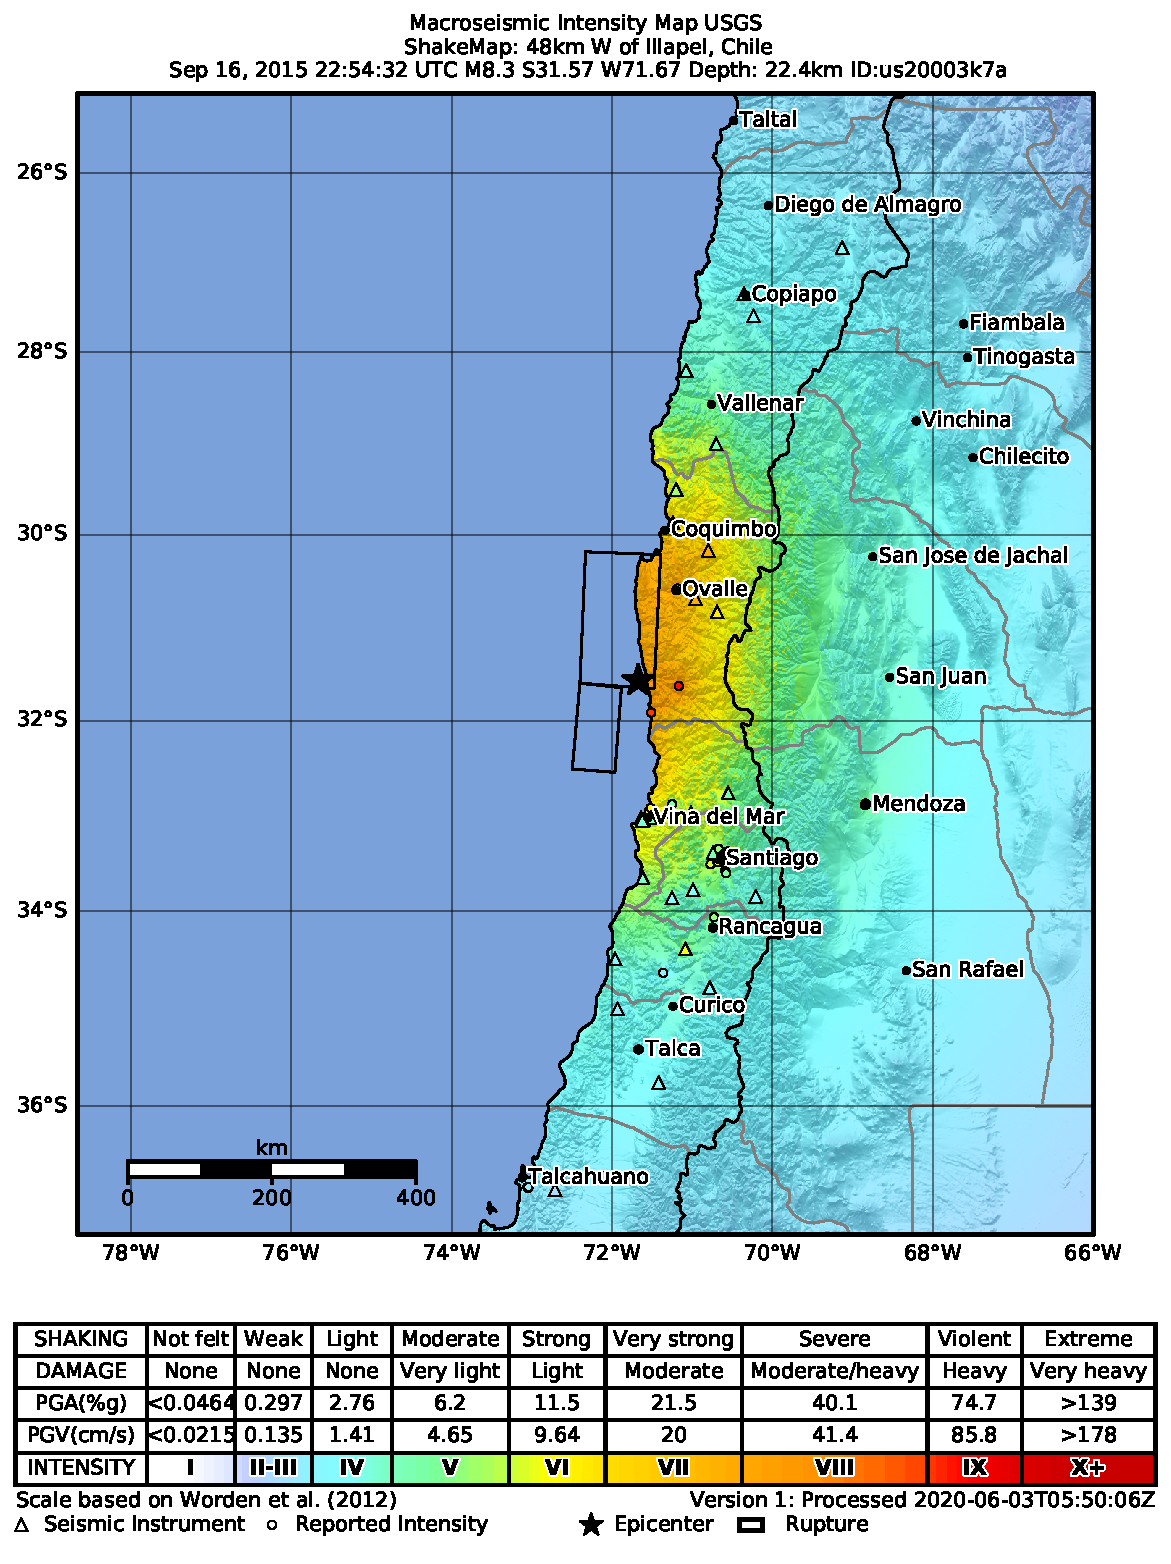
\includegraphics[width=0.7\textwidth]{Figures/intensity.pdf}
  \caption{Mapa de intensidades macrosísmicas (MMI) para el terremoto de Illapel 2015, basado en el ShakeMap del USGS \cite{USGS_ShakeMap_Illapel2015,Wikipedia_Illapel2015}.}
  \label{fig:intensity_illapel}
\end{figure}

\subsubsection{Mecanismo focal}

El mecanismo focal determinado por el USGS para el evento principal indica un movimiento de falla inversa sobre un plano de rumbo aproximadamente norte-sur (Figura \ref{fig:mecanismo_illapel}), consistente con movimientos de subducción entre las placas de Nazca y Sudamérica \cite{USGS_Illapel2015,IRIS_SpecialEvent_Illapel2015,Ruiz_SeismicSequence_Illapel2016}. Este mecanismo focal es típico de terremotos \emph{megathrust} en márgenes convergentes y explica la generación de importantes levantamientos cosísmicos y deformaciones asociadas en la zona costera \cite{Aranguiz_Geotech_Illapel2015,Ruiz_SeismicSequence_Illapel2016}.

\begin{figure}[h]
  \centering
  % Subfiguras horizontales: requiere \usepackage{subcaption}
  \begin{subfigure}[b]{0.48\textwidth}
    \centering
    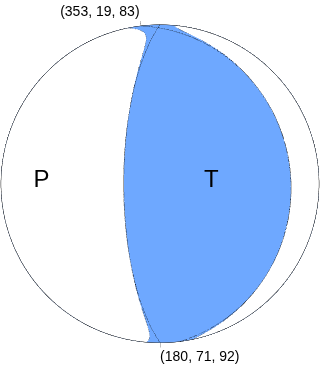
\includegraphics[width=0.7\textwidth]{Figures/mecanismo_focal.png}
    \caption{Mecanismo focal del terremoto de Illapel 2015 (Mw 8.3), según soluciones de momento tensor de USGS \cite{USGS_Illapel2015}.}
    \label{fig:mecanismo_illapel}
  \end{subfigure}
  \hfill
  \begin{subfigure}[b]{0.48\textwidth}
    \centering
    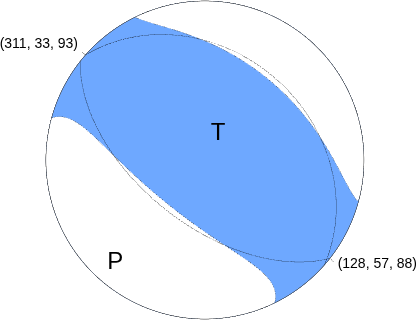
\includegraphics[width=\textwidth]{Figures/mecanismo_focal_2.png}
    \caption{Mecanismo focal del terremoto del Paso Drake 2025 (Mw 7.4), de acuerdo con la solución de falla inversa somera reportada por USGS \cite{USGS_Drake2025}.}
    \label{fig:mecanismo_drake}
  \end{subfigure}
  \caption{Mecanismos focales de los terremotos de Illapel 2015 (Mw 8.3) y Paso Drake 2025 (Mw 7.4), que ilustran el fallamiento inverso asociado al la región de subducción en el margen chileno y a la convergencia de placas en el Paso Drake \cite{USGS_Illapel2015,USGS_Drake2025}.}
  \label{fig:mecanismos_focales}
\end{figure}

\subsubsection{Otros datos relevantes}

El terremoto de Illapel 2015 generó un tsunami que fue registrado a lo largo de la costa central de Chile y en distintos mareógrafos del Pacífico \cite{IRIS_SpecialEvent_Illapel2015,ITIC_Tsunami_Illapel2015,Aranguiz_Geotech_Illapel2015}. En la estación de mareas de Coquimbo se midieron alturas de ola del orden de 4.75 m, mientras que en sectores cercanos al epicentro se reportaron run-ups máximos de aproximadamente 11 m sobre el nivel del mar \cite{Aranguiz_Geotech_Illapel2015,ITIC_Tsunami_Illapel2015}. La secuencia sísmica incluyó miles de réplicas, con al menos 31 eventos de magnitud mayor o igual a 6.0, que delinean el área de ruptura principal y su entorno inmediato en el interfaz de subducción \cite{Wikipedia_Illapel2015,Ruiz_SeismicSequence_Illapel2016}. Evaluaciones posteriores del daño indican que, pese a la alta magnitud, las intensidades observadas y el nivel de daño estructural fueron relativamente menores que lo esperado para un \emph{megathrust} de esta energía, lo que ha sido atribuido, entre otros factores, a las propiedades de sitio y a las características del movimiento fuerte registrado \cite{Fernandez_Damage_Illapel2018}.


\subsection{Características del terremoto del Paso Drake 2025 y razones de la alerta preventiva}

El terremoto del Paso Drake del 2 de mayo de 2025 corresponde a un evento de magnitud momento Mw 7.4, localizado por el USGS a las 12:58:26 UTC, con hipocentro en 56.809°S y 68.102°W y una profundidad de 10 km en la zona marítima entre el extremo sur de Sudamérica y la Antártica \cite{USGS_Drake2025,Wikipedia_Drake2025}. Esta configuración geométrica y la baja profundidad del evento lo clasifican como un sismo de falla inversa, capaz de generar perturbaciones significativas en el nivel del mar y, por tanto, potenciales tsunamis en las costas cercanas \cite{USGS_Drake2025}.

Desde el punto de vista tectónico, el evento ocurrió en una región de interacción donde convergen las placas Sudamericana, Antártica y Scotia, en las proximidades de un triple punto de placas \cite{USGS_Drake2025,Wikipedia_Drake2025}. La solución de mecanismo focal publicada por el USGS (Figura \ref{fig:mecanismo_drake}) indica un movimiento de compresión (falla inversa) sobre un plano de rumbo aproximado este--oeste, consistente con la convergencia relativa entre estas placas en el Paso Drake \cite{USGS_Drake2025,Wikipedia_Drake2025}. Esta combinación de alta magnitud, profundidad superficial y contexto tectónico convergente incrementó la preocupación por la posible generación de un tsunami que afectara tanto al territorio antártico chileno como a la región de Magallanes.

Poco después del sismo, el Centro de Alerta de Tsunamis del Pacífico (PTWC) emitió un boletín en el que se evaluó la amenaza de tsunami para el Paso Drake y zonas adyacentes, estimando alturas de ola de entre 1 y 3 metros por sobre el nivel de marea para partes de la costa de Chile y de 0.3 a 1 metro para sectores de la Antártica \cite{PTWC_Drake2025}. Aunque las amplitudes pronosticadas no representaban un peligro extremo, la incertidumbre asociada al modelo de tsunami y la presencia de instalaciones científicas y militares en la zona motivaron una respuesta precautoria de las autoridades competentes \cite{PTWC_Drake2025,USAToday_Drake2025,CGTN_Drake2025}.

En Chile, el Servicio Nacional de Prevención y Respuesta ante Desastres (SENAPRED) y el Servicio Hidrográfico y Oceanográfico de la Armada (SHOA) declararon un estado de alerta preventiva (estado de precaución) para el borde costero de la región de Magallanes y para el territorio antártico, ordenando la evacuación de zonas de playa y la movilización hacia áreas seguras \cite{DW_Drake2025,Reuters_Drake2025,USAToday_Drake2025}. Informes de noticieros locales indican que se evacuaron alrededor de 2\,000 personas en sectores costeros del extremo sur, mientras que en bases antárticas se mantuvo el monitoreo del nivel del mar y la aplicación de protocolos de emergencia \cite{DW_Drake2025,Reuters_Drake2025}.

En síntesis, las características especiales que hicieron que el terremoto del Paso Drake de 2025 generara una alerta preventiva fueron su alta magnitud (Mw 7.4), la profundidad superficial (\(\sim 10\) km), su ubicación en un contexto de convergencia de placas cercano a un triple punto, la posibilidad modelada de alturas de tsunami de hasta 1--3 m en zonas costeras de Chile y la presencia de instalaciones sensibles en la región de Magallanes y en la Antártica chilena \cite{USGS_Drake2025,PTWC_Drake2025,Reuters_Drake2025,Wikipedia_Drake2025}.


\subsection{¿Liberó el terremoto de Iquique 2014 toda la energía acumulada? Discusión}

El terremoto de Iquique del 1 de abril de 2014 (Mw 8.1--8.2) ocurrió dentro de la región sísmica del norte de Chile, un segmento de subducción que no tenía un gran megaterremoto desde el evento de 1877 (Mw $\sim$ 8.8) \cite{USGS_Iquique2014,Hayes_Iquique2014}. Diversos estudios que combinan sismología, geodesia (GPS e InSAR) y modelos de tsunami muestran que la ruptura de 2014 afectó sólo una parte de la región, lo que implica que no se liberó toda la energía acumulada en el sistema durante siglos \cite{Hayes_Iquique2014,Duputel_Iquique2015,Watada_Iquique2014}.

El análisis de la distribución de deslizamiento cosísmico reveló que la ruptura principal de Iquique fue relativamente reducida, con un área del orden de 100 km $\times$ 50 km y desplazamientos máximos cercanos a 7 m \cite{Duputel_Iquique2015,Watada_Iquique2014}. A su vez, estudios de modelo de falla finita y de ondas de tsunami indican que la zona de mayor desplazamiento se restringe a una porción central de la región de subducción, mientras que grandes segmentos al norte y al sur permanecen sin un deslizamiento significativo \cite{Watada_Iquique2014}. Esto es consistente con modelos de acoplamiento intersísmico basados en GPS, que muestran segmentos altamente trabados (\textit{“highly locked”}) circundantes a la región que se desplazó en 2014 y que podrían albergar futuros megaterremotos \cite{Metois_NorthChileGap2013,Hayes_Iquique2014}.

Otro argumento que respalda la idea de que el terremoto de Iquique no liberó toda la energía acumulada proviene de la estimación del déficit de momento\footnote{La diferencia acumulada entre la energía o el desplazamiento que las placas tectónicas deberían liberar teóricamente en una falla} y de la segmentación de la falla \cite{Hayes_Iquique2014,Schurr_IquiqueGap2014}. Los resultados sugieren que el desplazamiento del 2014 afectó del orden de un 20--30\% de la extensión total de la falla, dejando secciones con acoplamiento fuerte que podrían producir eventos con magnitudes potenciales mayores que 8.5 en el futuro \cite{Hayes_Iquique2014}. Además, modelos que consideraron la geometría de la placa de Nazca y la presencia de zonas de acoplamiento reducido indican que ciertas regiones actúan como barreras naturales que limitaron la propagación de la ruptura de Iquique, favoreciendo una liberación parcial del esfuerzo acumulado en la zona \cite{Metois_NorthChileGap2013,Schurr_IquiqueGap2014}.  Se ha propuesto que dichas barreras naturales incluyen relieves en la placa de Nazca, como montes submarinos \cite{Geersen_Seamounts2016}.

Sobre la pregunta de si es posible “saber” que no se liberó toda la energía, la respuesta es complicada. En la práctica, lo que se estima no es directamente la energía, sino el déficit de energía liberada respecto al esperado por modelos teóricos que se actualizan con el tiempo \cite{Metois_NorthChileGap2013,Hayes_Iquique2014}. Por lo tanto, las incertidumbres asociadas a dichos modelos y la contribución de las barreras naturales en la liberación de energía impiden afirmar con exactitud cuánta energía permanece almacenada y en qué momento podría liberarse \cite{Nucleation_Iquique2016,Eskp_IquiqueHazard2014}.  En resumen, la afirmación de que el terremoto de Iquique 2014 no liberó toda la energía acumulada se basa en evidencia cuantitativa sólida \cite{Hayes_Iquique2014,Duputel_Iquique2015}. No obstante, la imposibilidad actual de medir directamente el estado de los esfuerzos en las placas y de capturar todo el relieve del fondo marino hace que esta conclusión sea necesariamente probabilística y dependiente de los modelos \cite{Cesca_Iquique2016,Eskp_IquiqueHazard2014,USGS_Iquique2014}.


\subsection{Clasificación de la sismicidad en la región seleccionada de Chile}
Para la construcción del catálogo sísmico seleccioné como región de estudio el segmento de subducción Coquimbo--Illapel en los años 2007 a 2017, delimitado aproximadamente entre latitudes $29^\circ S$ y $33^\circ S$ y longitudes $69^\circ W$ y $73^\circ W$, abarcando profundidades entre 0 y 60 km, de modo que se incluya el megaterremoto de Illapel del 16 de septiembre de 2015 (Mw 8.3) y la sismicidad interplaca asociada al contacto entre las placas de Nazca y Sudamérica. El catálogo resultante contiene un total de 2563 eventos sísmicos, con magnitudes entre 2.5 y 8.3 cuya distribución espacial se encuentra representada en la Figura \ref{fig:seismicity}.

\clearpage

\begin{figure}
\centering
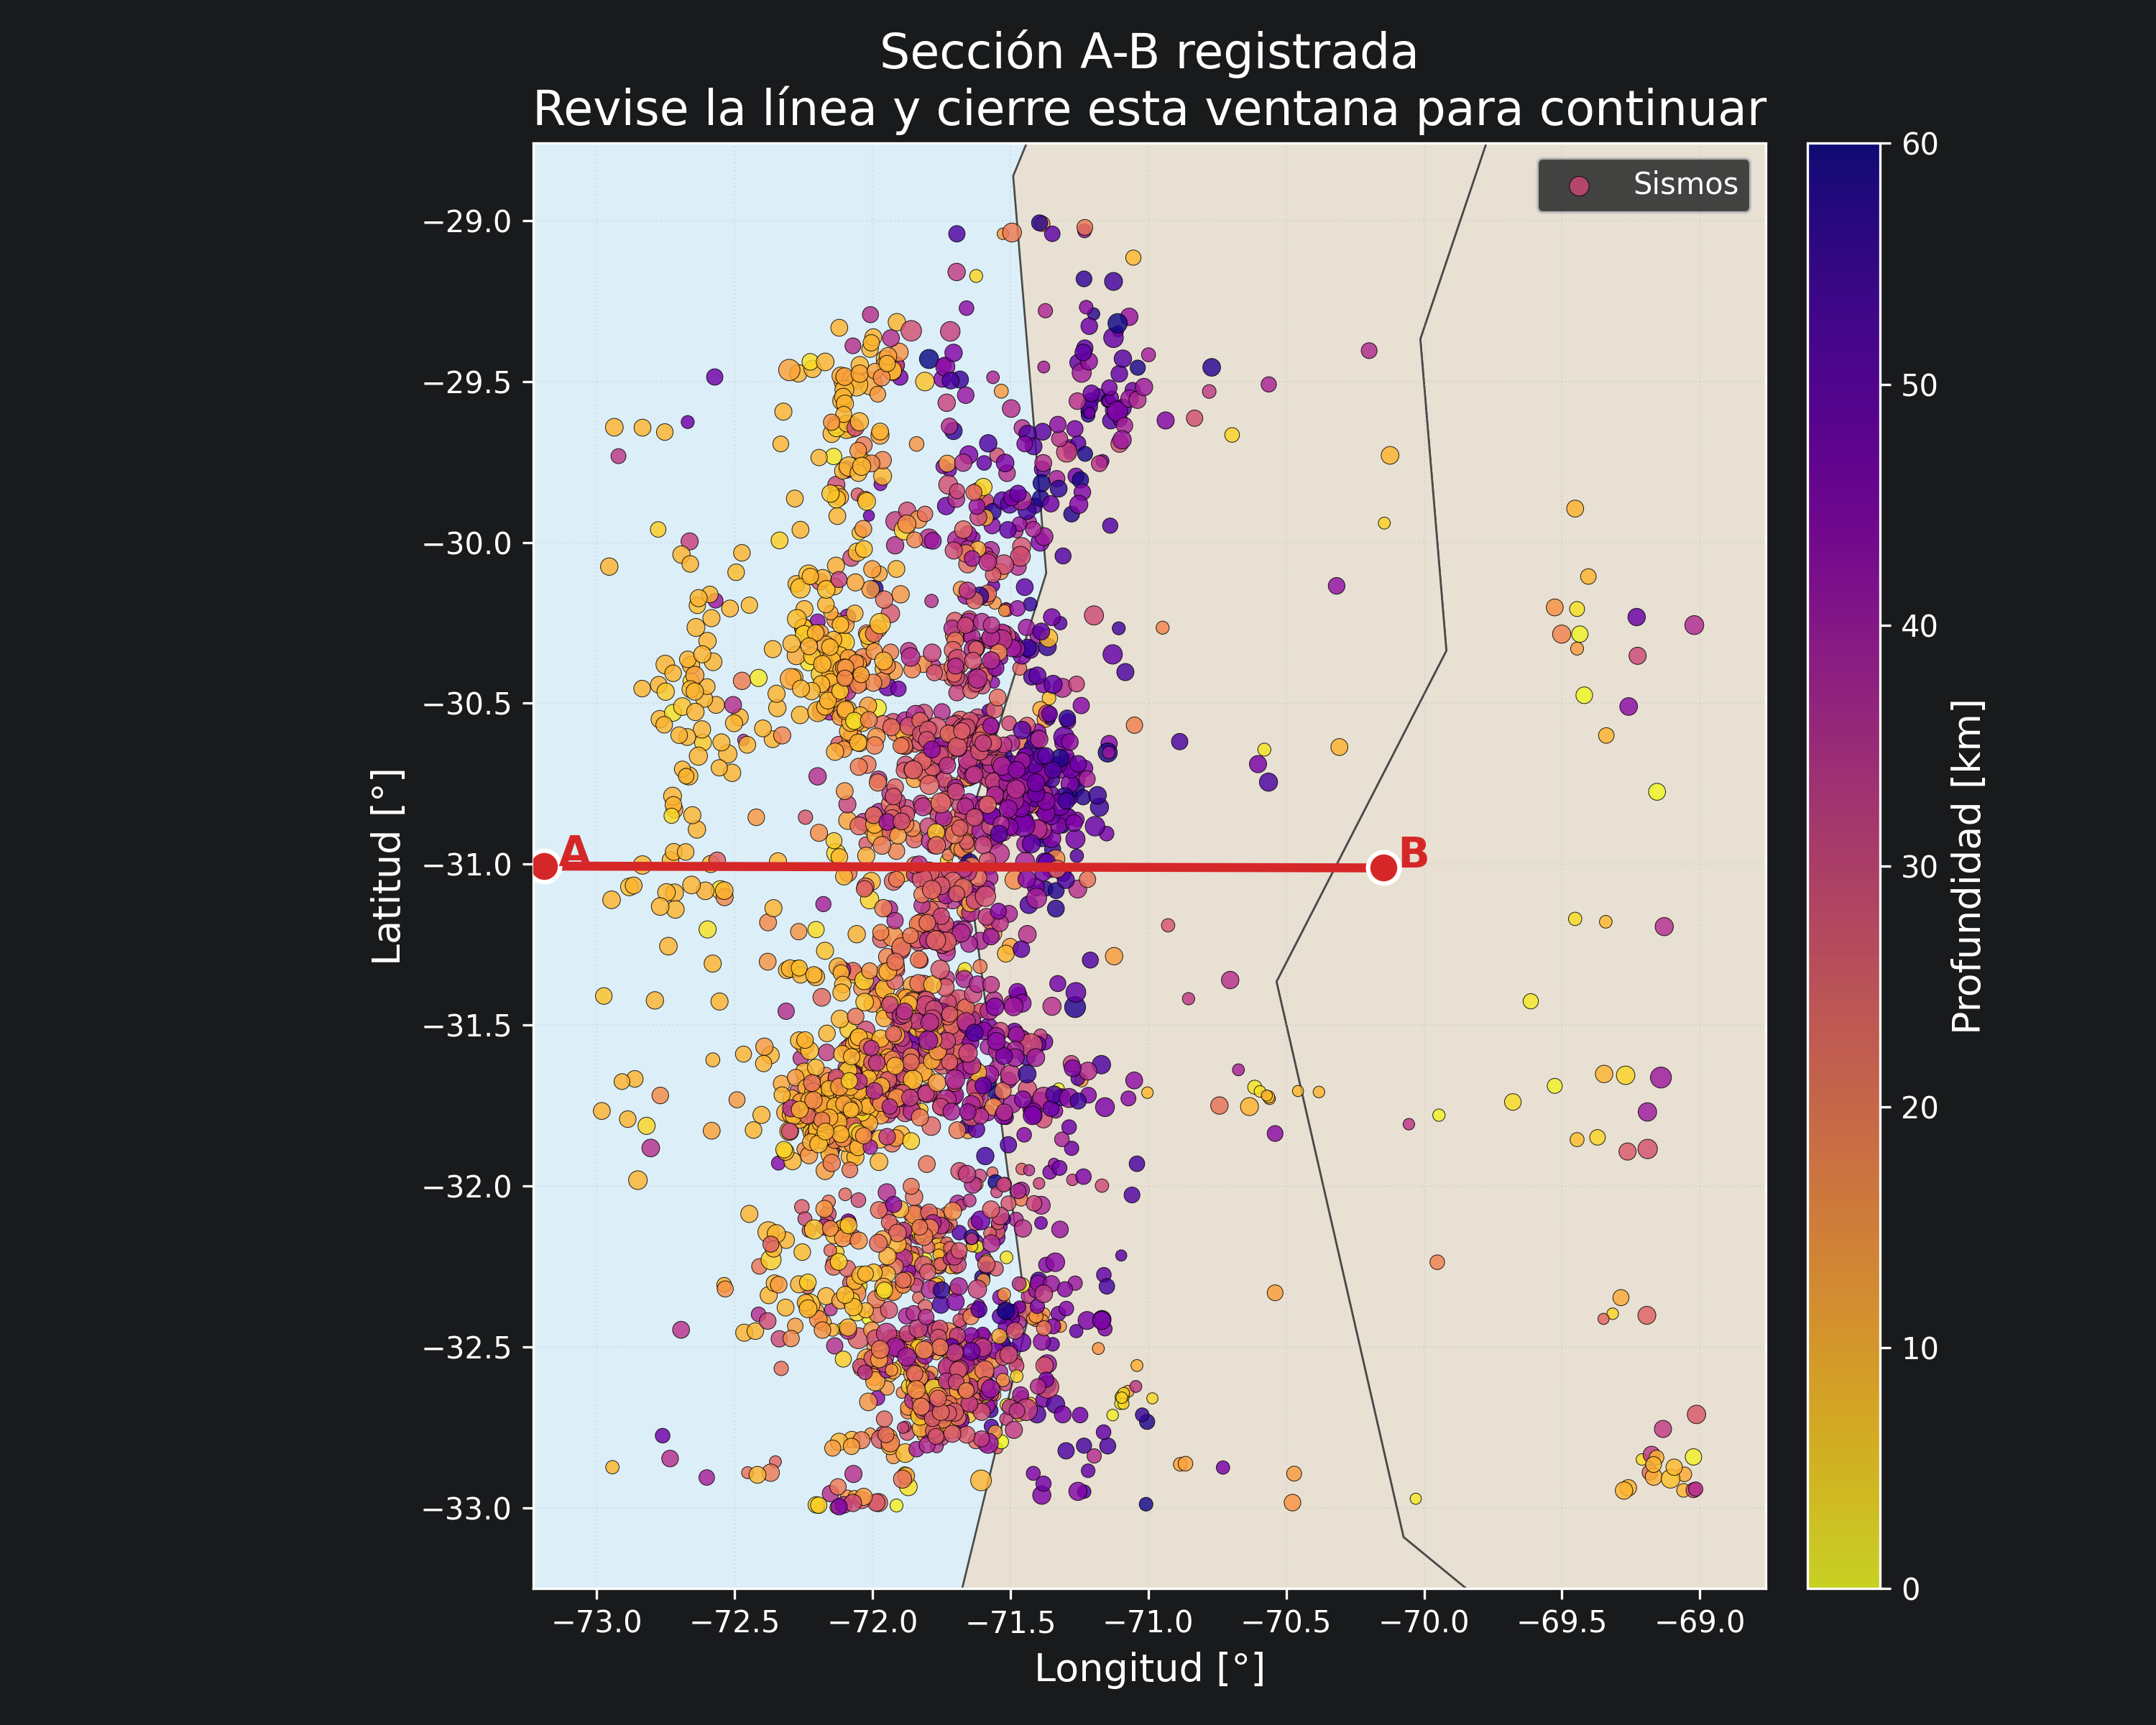
\includegraphics[width=\textwidth]{Figures/Seccion_elegida}
\caption{Distribución espacial de la sismicidad en la región de estudio. Los puntos A y B representan los extremos de la sección transversal utilizada para el perfil de profundidad. La densidad de eventos es mayor cerca de la costa, disminuyendo hacia el interior del continente.}
\label{fig:seismicity}
\end{figure}

\begin{figure}
\centering
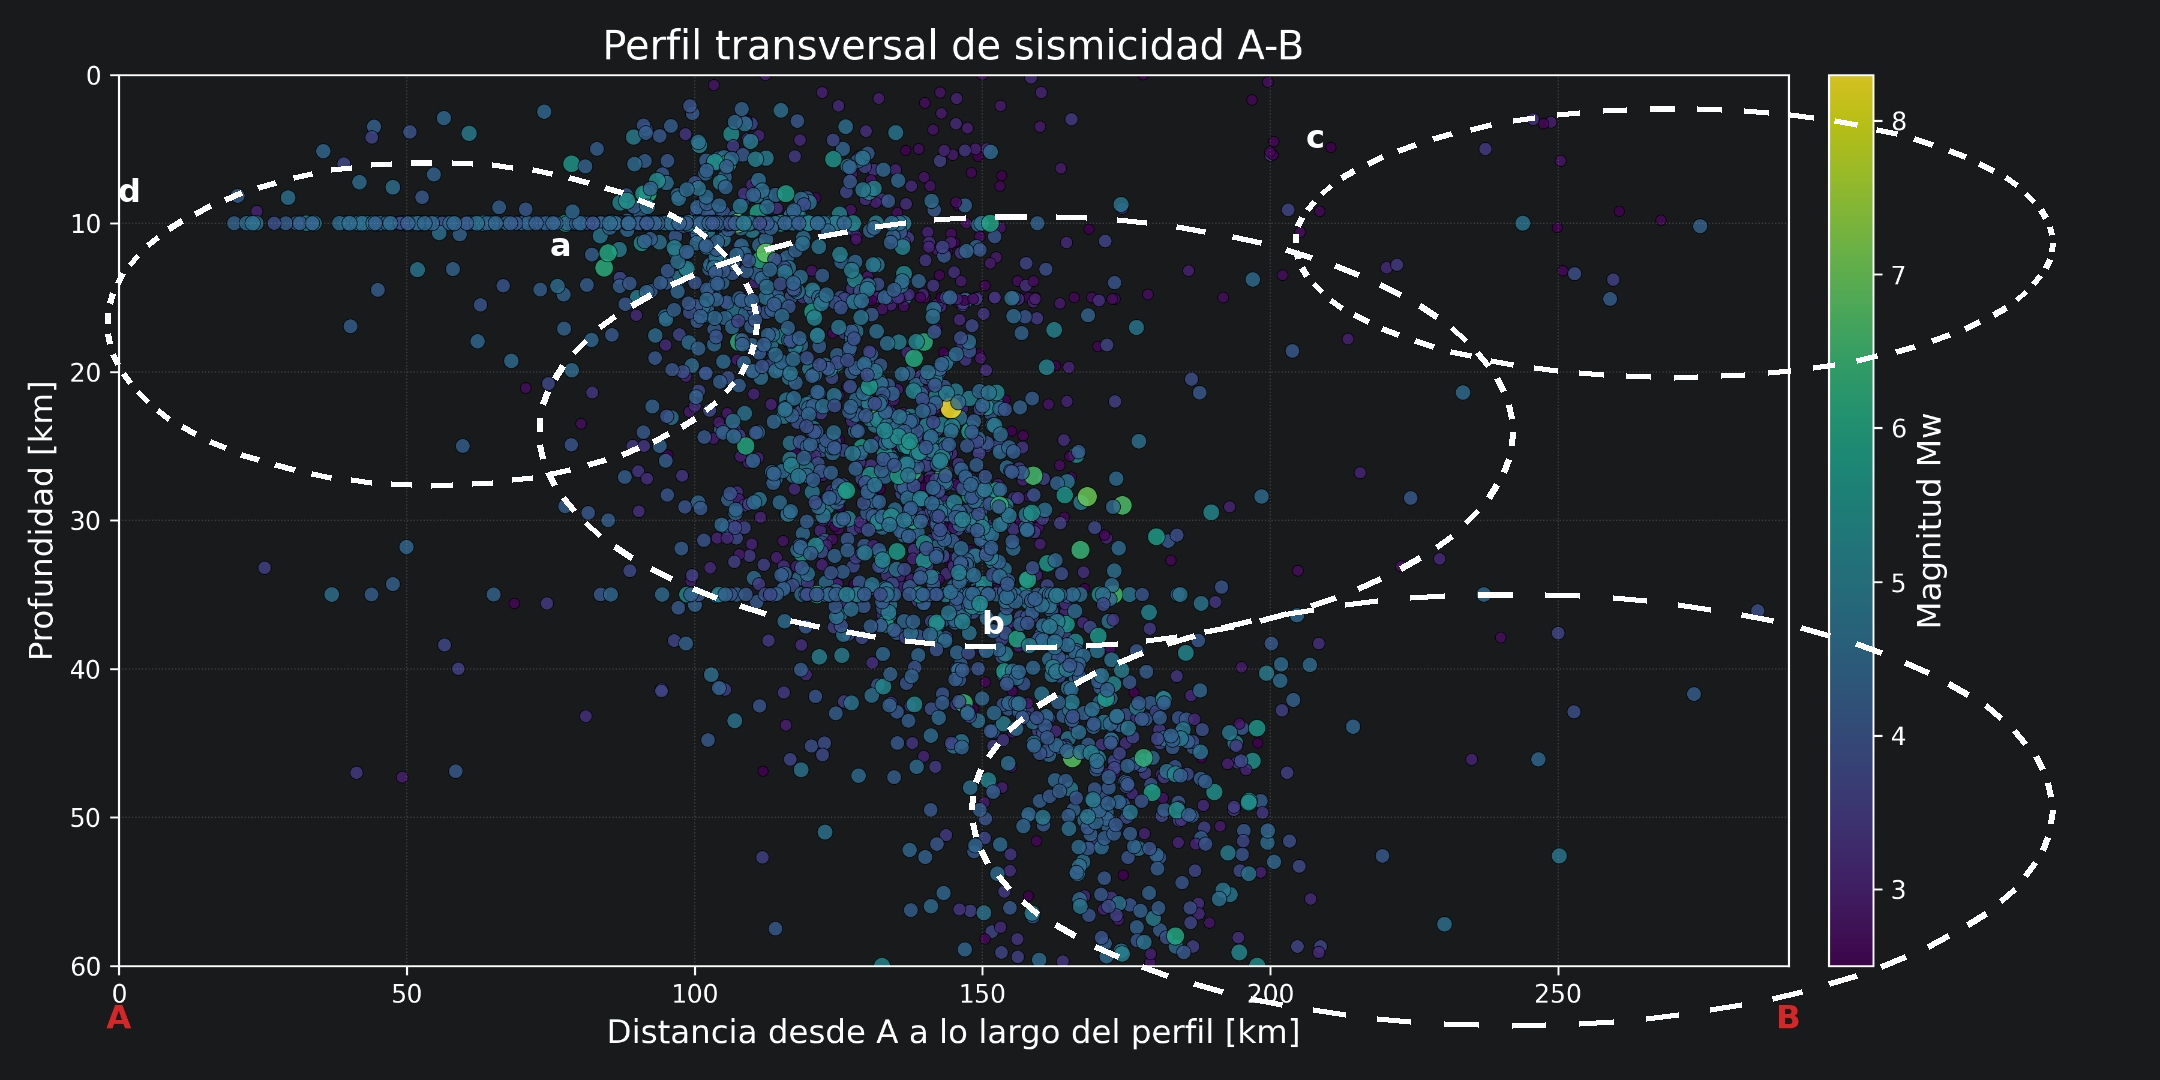
\includegraphics[width=\textwidth]{Figures/Perfil_AB_clasificado}
\caption{Perfil de profundidad de la sismicidad en la región de estudio. Los elipsoides representan las diferentes tipologías de terremotos según la profundidad del punto focal.}
\label{fig:depth_profile}
\end{figure}

En la figura \ref{fig:seismicity} se observa que la sismicidad se concentra principalmente a lo largo de la zona de subducción, con una densidad mayor de eventos en el área costera y una disminución progresiva hacia el interior del continente. Para ahondar más en la distribución de la sismicidad, la Figura \ref{fig:depth_profile} muestra un perfil de profundidad a lo largo de la sección A--B, donde se aprecia la inclinación del plano de subducción y la concentración de eventos a profundidades intermedias, típicas de sismos interplaca. A su vez, se reconocen y resaltan como elipses blancas cuatro dominios principales de sismicidad: interplaca, intraplaca oceánica de profundidad intermedia, cortical continental y \emph{outer--rise} oceánica \cite{fernandez_2018}. Cada uno se asocia a procesos tectónicos específicos controlados por la convergencia entre las placas de Nazca y Sudamericana, que ocurre a una velocidad del orden de 66~mm/año a lo largo de este margen \cite{csn_tipos_sismos}. Las siguientes subsecciones describen brevemente cada tipología de sismos identificada en la región de estudio.

\subsubsection{Sismicidad interplaca (megathrust)}

En el perfil transversal A--B de la Figura \ref{fig:depth_profile} se observa una banda bien definida de eventos que sigue un plano inclinado desde profundidades cercanas a 10--20~km bajo la costa hasta alrededor de 50--60~km mar adentro; dicha banda corresponde a la zona de acoplamiento interplaca entre las placas Nazca y Sudamericana, donde se generan los grandes terremotos de subducción \cite{fernandez_2018, csn_tipos_sismos}. De acuerdo con la clasificación del Centro Sismológico Nacional (CSN), estos sismos interplaca son predominantemente compresionales, con mecanismos de falla inversa, y se concentran en profundidades menores a aproximadamente 40--60~km; su magnitud está controlada por el área de ruptura y el desplazamiento en la región \cite{csn_tipos_sismos}.

Tectónicamente, esta sismicidad refleja la liberación del esfuerzo compresivo acumulado en la zona de contacto entre las placas, donde el acoplamiento mecánico traba el movimiento relativo de las placas hasta que se supera la resistencia friccional y se produce un deslizamiento súbito del plano de subducción \cite{csn_tipos_sismos,fernandez_2018}. Los eventos de gran magnitud en este dominio pueden generar importantes levantamientos del fondo oceánico y, por tanto, tsunamis asociados. Ejemplos de este tipo de sismos son el terremoto de Valdivia de 1960 ($M_w=9.5$) y el terremoto del Maule del 2010 ($M_w=8.8$).

\subsubsection{Sismicidad intraplaca oceánica de profundidad intermedia}

Por debajo de la región de interplaca, el perfil muestra otra concentración de sismos distribuidos dentro de la placa de Nazca en profundidades típicamente entre 50 y 250~km, siguiendo la prolongación del \emph{slab} hacia el interior de la litosfera oceánica \cite{fernandez_2018, csn_tipos_sismos}. Estos eventos se clasifican como sismos intraplaca de profundidad intermedia, al ocurrir dentro de la placa oceánica ya subducida, por encima de la profundidad donde se estima que la placa pierde su comportamiento frágil \cite{csn_tipos_sismos}.

Los procesos tectónicos que sustentan esta sismicidad incluyen la deformación interna de la placa debido a cambios de fase mineralógicos, variaciones en el régimen de esfuerzos y fuerzas de flexión y tracción asociadas al hundimiento de la placa en el manto \cite{csn_tipos_sismos}. Se ha observado que estos sismos intraplaca pueden tener un potencial de daño mayor que los interplaca de magnitud similar, dado que su profundidad intermedia favorece una concentración de energía sísmica efectiva en áreas pobladas \cite{csn_tipos_sismos}.

\subsubsection{Sismicidad cortical continental}

En el extremo continental de perfil de la Figura \ref{fig:depth_profile}, cercano a la superficie, se observa una población de eventos aislados que se ubican dentro de la corteza de la placa Sudamericana, a profundidades menores a aproximadamente 60~km y asociados a estructuras corticales internas. Estos sismos corresponden a la categoría de sismos superficiales o corticales, definidos por el CSN como eventos que ocurren dentro de la placa continental y están ligados a las deformaciones generadas por la convergencia Nazca--Sudamericana y al levantamiento de la Cordillera de los Andes \cite{csn_tipos_sismos}.

Tectónicamente, la sismicidad cortical refleja el ajuste de la corteza a la carga y a los esfuerzos transmitidos desde el contacto interplaca, expresándose en fallas de la corteza superior e inferior que acomodan el relieve y área de la región \cite{csn_tipos_sismos,fernandez_2018}. Ejemplos de este tipo incluyen terremotos históricos como el de Las Melosas, que muestran cómo la deformación cortical puede generar sismos dañinos en la región.

\subsubsection{Sismicidad \emph{outer--rise} e intraplaca oceánica aislada}

Hacia el lado oceánico, por delante de la fosa, el perfil y la proyección en planta evidencian un conjunto de sismos someros ubicados costa afuera, en la zona de máxima curvatura de la placa de Nazca antes de iniciar la subducción (región superior izquierda, Figura \ref{fig:depth_profile}). Estos eventos se clasifican como sismos \emph{outer--rise}. Según la descripción del CSN, los sismos \emph{outer--rise} ocurren típicamente a profundidades menores de 30~km, en la región donde la placa oceánica se flexiona para ingresar en la fosa; su magnitud suele ser menor que 7{,}0 y en general no generan tsunamis significativos \cite{csn_tipos_sismos}.

Los procesos tectónicos que sustentan estos eventos están relacionados con la flexión de la placa oceánica, que genera un campo de esfuerzos extensional por encima y compresivo por debajo de la zona de curvatura, activando fallas normales e inversas dentro de la litosfera oceánica.

\subsection{Patrones temporales y espaciales de la sismicidad}

Con el propósito de examinar la evolución espacio--temporal de la actividad sísmica en la región seleccionada, la Figura~\ref{fig:perfil-temporal} presenta la distribución de los eventos en función de la latitud y el tiempo durante el período 2007--2017. El diagrama central permite identificar concentraciones latitudinales y cambios en la tasa de ocurrencia, mientras que el histograma superior representa el número de eventos a lo largo del tiempo y el histograma lateral resume su distribución por latitud. El color de cada punto corresponde a su profundidad, lo que facilita distinguir la ocurrencia relativa de sismos superficiales e intermedios dentro del rango de tiempo seleccionado.

\begin{figure}[htbp]
    \centering
    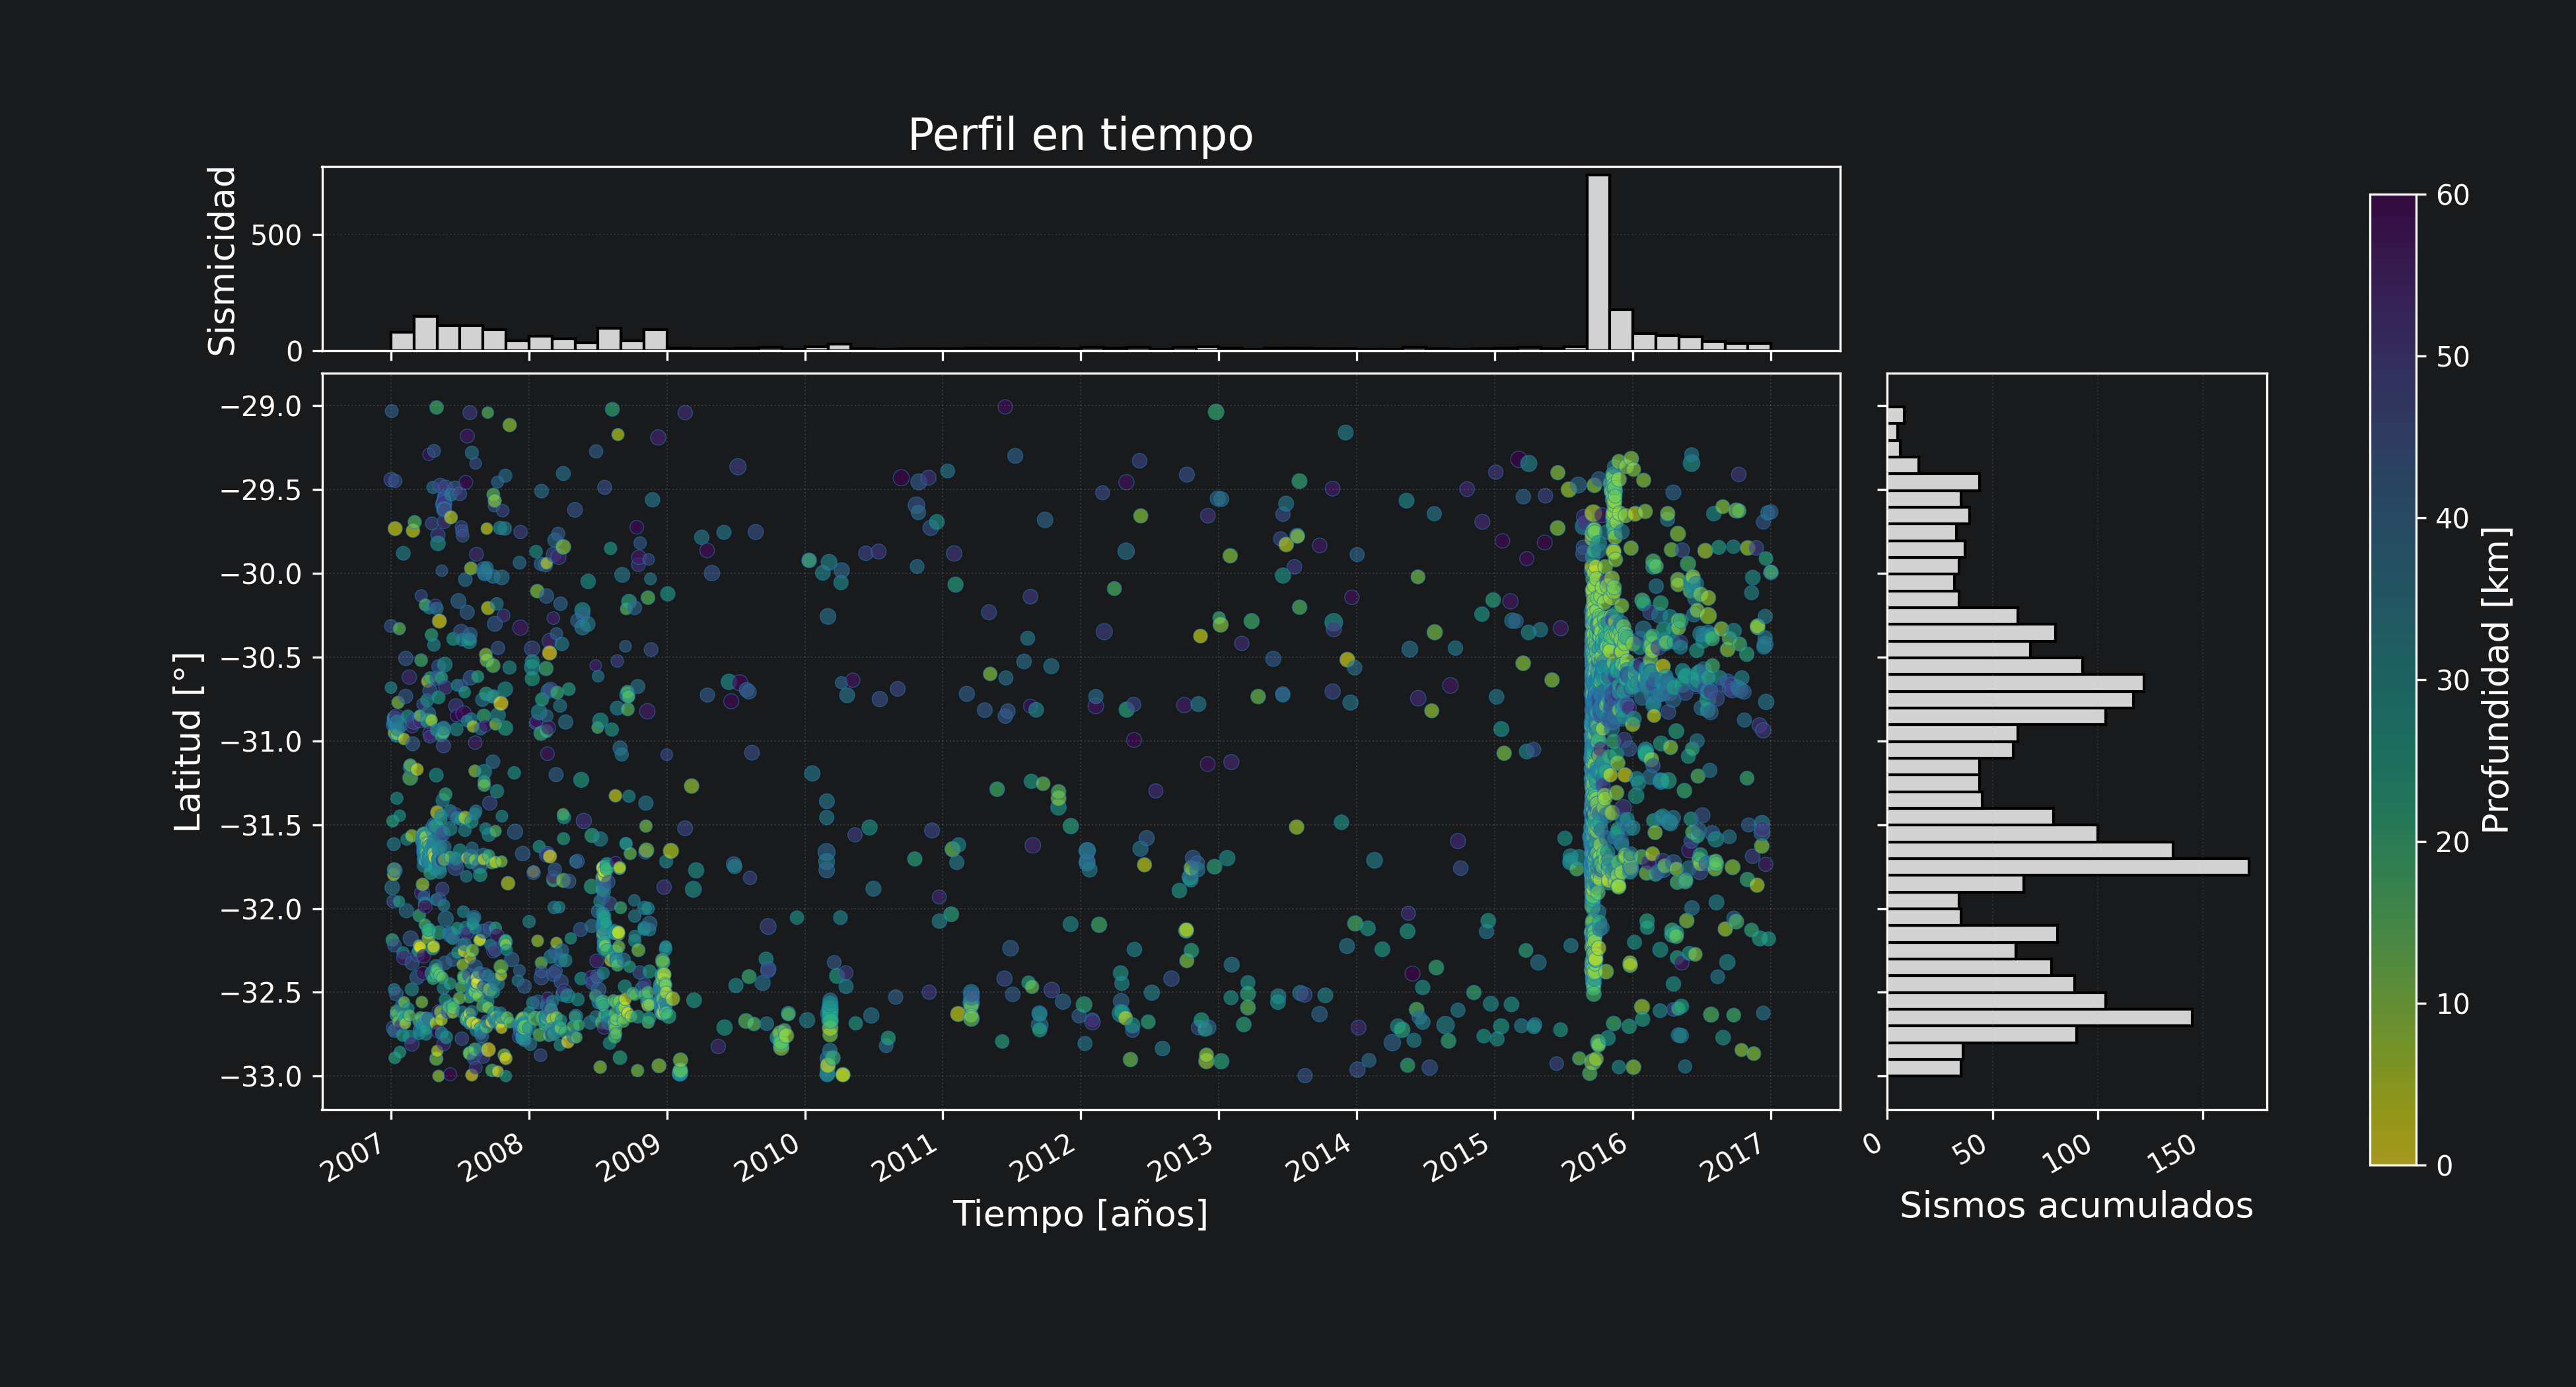
\includegraphics[width=\textwidth]{Figures/Perfil_Temporal}
    \caption{Distribución espacio--temporal de la sismicidad en la región de estudio entre 2007 y 2017. El panel central muestra la latitud de los eventos en función del tiempo, coloreado por la profundidad focal en kilómetros. El histograma superior representa el número de eventos por intervalo temporal y el histograma lateral representa el número acumulado de eventos según la latitud.}
    \label{fig:perfil-temporal}
\end{figure}

El gráfico de latitud versus tiempo evidencia una sismicidad altamente marcada durante el período 2007--2017. La mayor parte del registro corresponde a actividad de fondo, relativamente dispersa y de menor frecuencia (años 2009 a 2015 principalmente), mientras que entre septiembre de 2015 y comienzos de 2016 se observa un incremento abrupto y dominante del número de eventos, reflejado tanto en la nube densa de puntos como en el máximo del histograma temporal.

La concentración principal de actividad ocurre en torno a septiembre de 2015, con una tasa de eventos considerablemente superior a la observada en los años anteriores y posteriores. Este patrón es coherente con la secuencia originada por el terremoto de Illapel del 16 de septiembre de 2015, cuyo evento principal tuvo magnitud Mw~8{,}3, se localizó aproximadamente a $31{,}57^\circ$S y $71{,}67^\circ$W, y ocurrió a una profundidad cercana a 22{,}4~km \cite{USGS_Illapel2015}.

Adicionalmente, se puede evidenciar que la secuencia posterior incluye una gran cantidad de réplicas, visibles como una banda casi vertical en el diagrama latitud--tiempo, que se prolonga desde fines de 2015 hasta parte de 2016. El máximo del histograma corresponde al inicio de esta secuencia, seguido por una disminución progresiva de la tasa sísmica, comportamiento que, como veremos más adelante, es compatible con la relajación temporal descrita por la ley de Omori \cite{utsu_1995}. El CSN reportó que, durante el primer año posterior al terremoto de Illapel, se registraron 4.220 réplicas de magnitud superior a 3, confirmando que el fuerte aumento observado no representa una variación aleatoria de la actividad de fondo, sino una secuencia de réplicas bien definida.

\subsubsection{Patrones espaciales y posible migración}

De la Figura \ref{fig:perfil-temporal}, se observa que, antes de 2015, la sismicidad se distribuye principalmente entre aproximadamente $29^\circ$S y $33^\circ$S, aunque se distinguen concentraciones persistentes en torno a $31{,}5^\circ$S--$32{,}0^\circ$S y en el extremo sur del catálogo, cercano a $32{,}5^\circ$S--$33^\circ$S (región inferior izquierda). Durante el evento de Illapel del 2015, la actividad se concentra preferentemente entre $29{,}5^\circ$S y $32{,}5^\circ$S, con un cluster importante alrededor de la latitud del evento principal, aproximadamente $31{,}6^\circ$S.

Estos indicios hallados en la figura \ref{fig:perfil-temporal} sugiere una expansión espacial de la secuencia desde el área de ruptura principal hacia segmentos adyacentes del margen, con réplicas distribuidas tanto al norte como al sur del epicentro del evento de Illapel. Esta geometría es consistente con la redistribución de esfuerzos estáticos y dinámicos producida por una ruptura de tal magnitud, que puede activar fallas cercanas y generar sismos en zonas previamente menos activas.

En particular, esta redistribución se aprecia principalmente como una actividad posterior en el sector sur de la zona analizada, cercano a $32^\circ$S--$33^\circ$S, la cual puede corresponder a la activación de estructuras adyacentes o a réplicas localizadas fuera de la zona de máximo deslizamiento.

Finalmente, la Figura~\ref{fig:perfil-temporal} muestra períodos de menor actividad sísmica antes del incremento abrupto registrado en septiembre de 2015. Entre 2010 y mediados de 2015, el número de eventos es considerablemente inferior al observado durante 2007--2009 y, especialmente, al de la secuencia posterior al terremoto de Illapel. En este sentido, es claro identificar una fase intersísmica, durante la cual la interacción entre placas puede permanecer parcial o fuertemente acoplada y acumular deformación elástica, junto con una fase cosísmica, caracterizada por la liberación súbita de dicha deformación durante un gran terremoto y una fase postsísmica, dominada por réplicas relacionadas a dicho evento.

\subsection{Relación entre la fosa, la costa y el peligro sísmico}

La comparación entre la ubicación de la fosa oceánica, la línea de costa (Figura \ref{fig:seismicity}) y el perfil de profundidad A--B (Figura \ref{fig:depth_profile}) permite inferir que la mayor concentración de sismicidad se localiza en el margen continental, entre el sector marino próximo a la costa y el continente inmediato.

En este sentido, la fosa representa la zona donde comienza el descenso de la placa oceánica. Hacia el este, bajo la zona costera, se concentra una parte importante de los eventos superficiales e intermedios. Por lo tanto, las localidades costeras se encuentran próximas a la proyección de la región interplaca, donde pueden ocurrir terremotos de gran magnitud~\cite{csn_tipos_sismos}.

Esta relación incrementa el peligro sísmico local de las zonas costeras, ya que su cercanía a las regiones interplaca puede producir movimientos fuertes del terreno durante grandes terremotos. Adicionalmente, si un evento de esta zona genera desplazamiento vertical del fondo marino, las localidades del borde costero están expuestas a un peligro complementario de tsunami. Por consiguiente, el peligro sísmico costero debe evaluarse considerando simultáneamente la distancia a la zona de ruptura, la profundidad de los eventos, las condiciones locales del suelo y la posible inundación asociada a tsunamis.

\section{Leyes Empíricas}
\subsection{Ley de Gutenberg-Richter}

\begin{figure}[h]
    \centering
    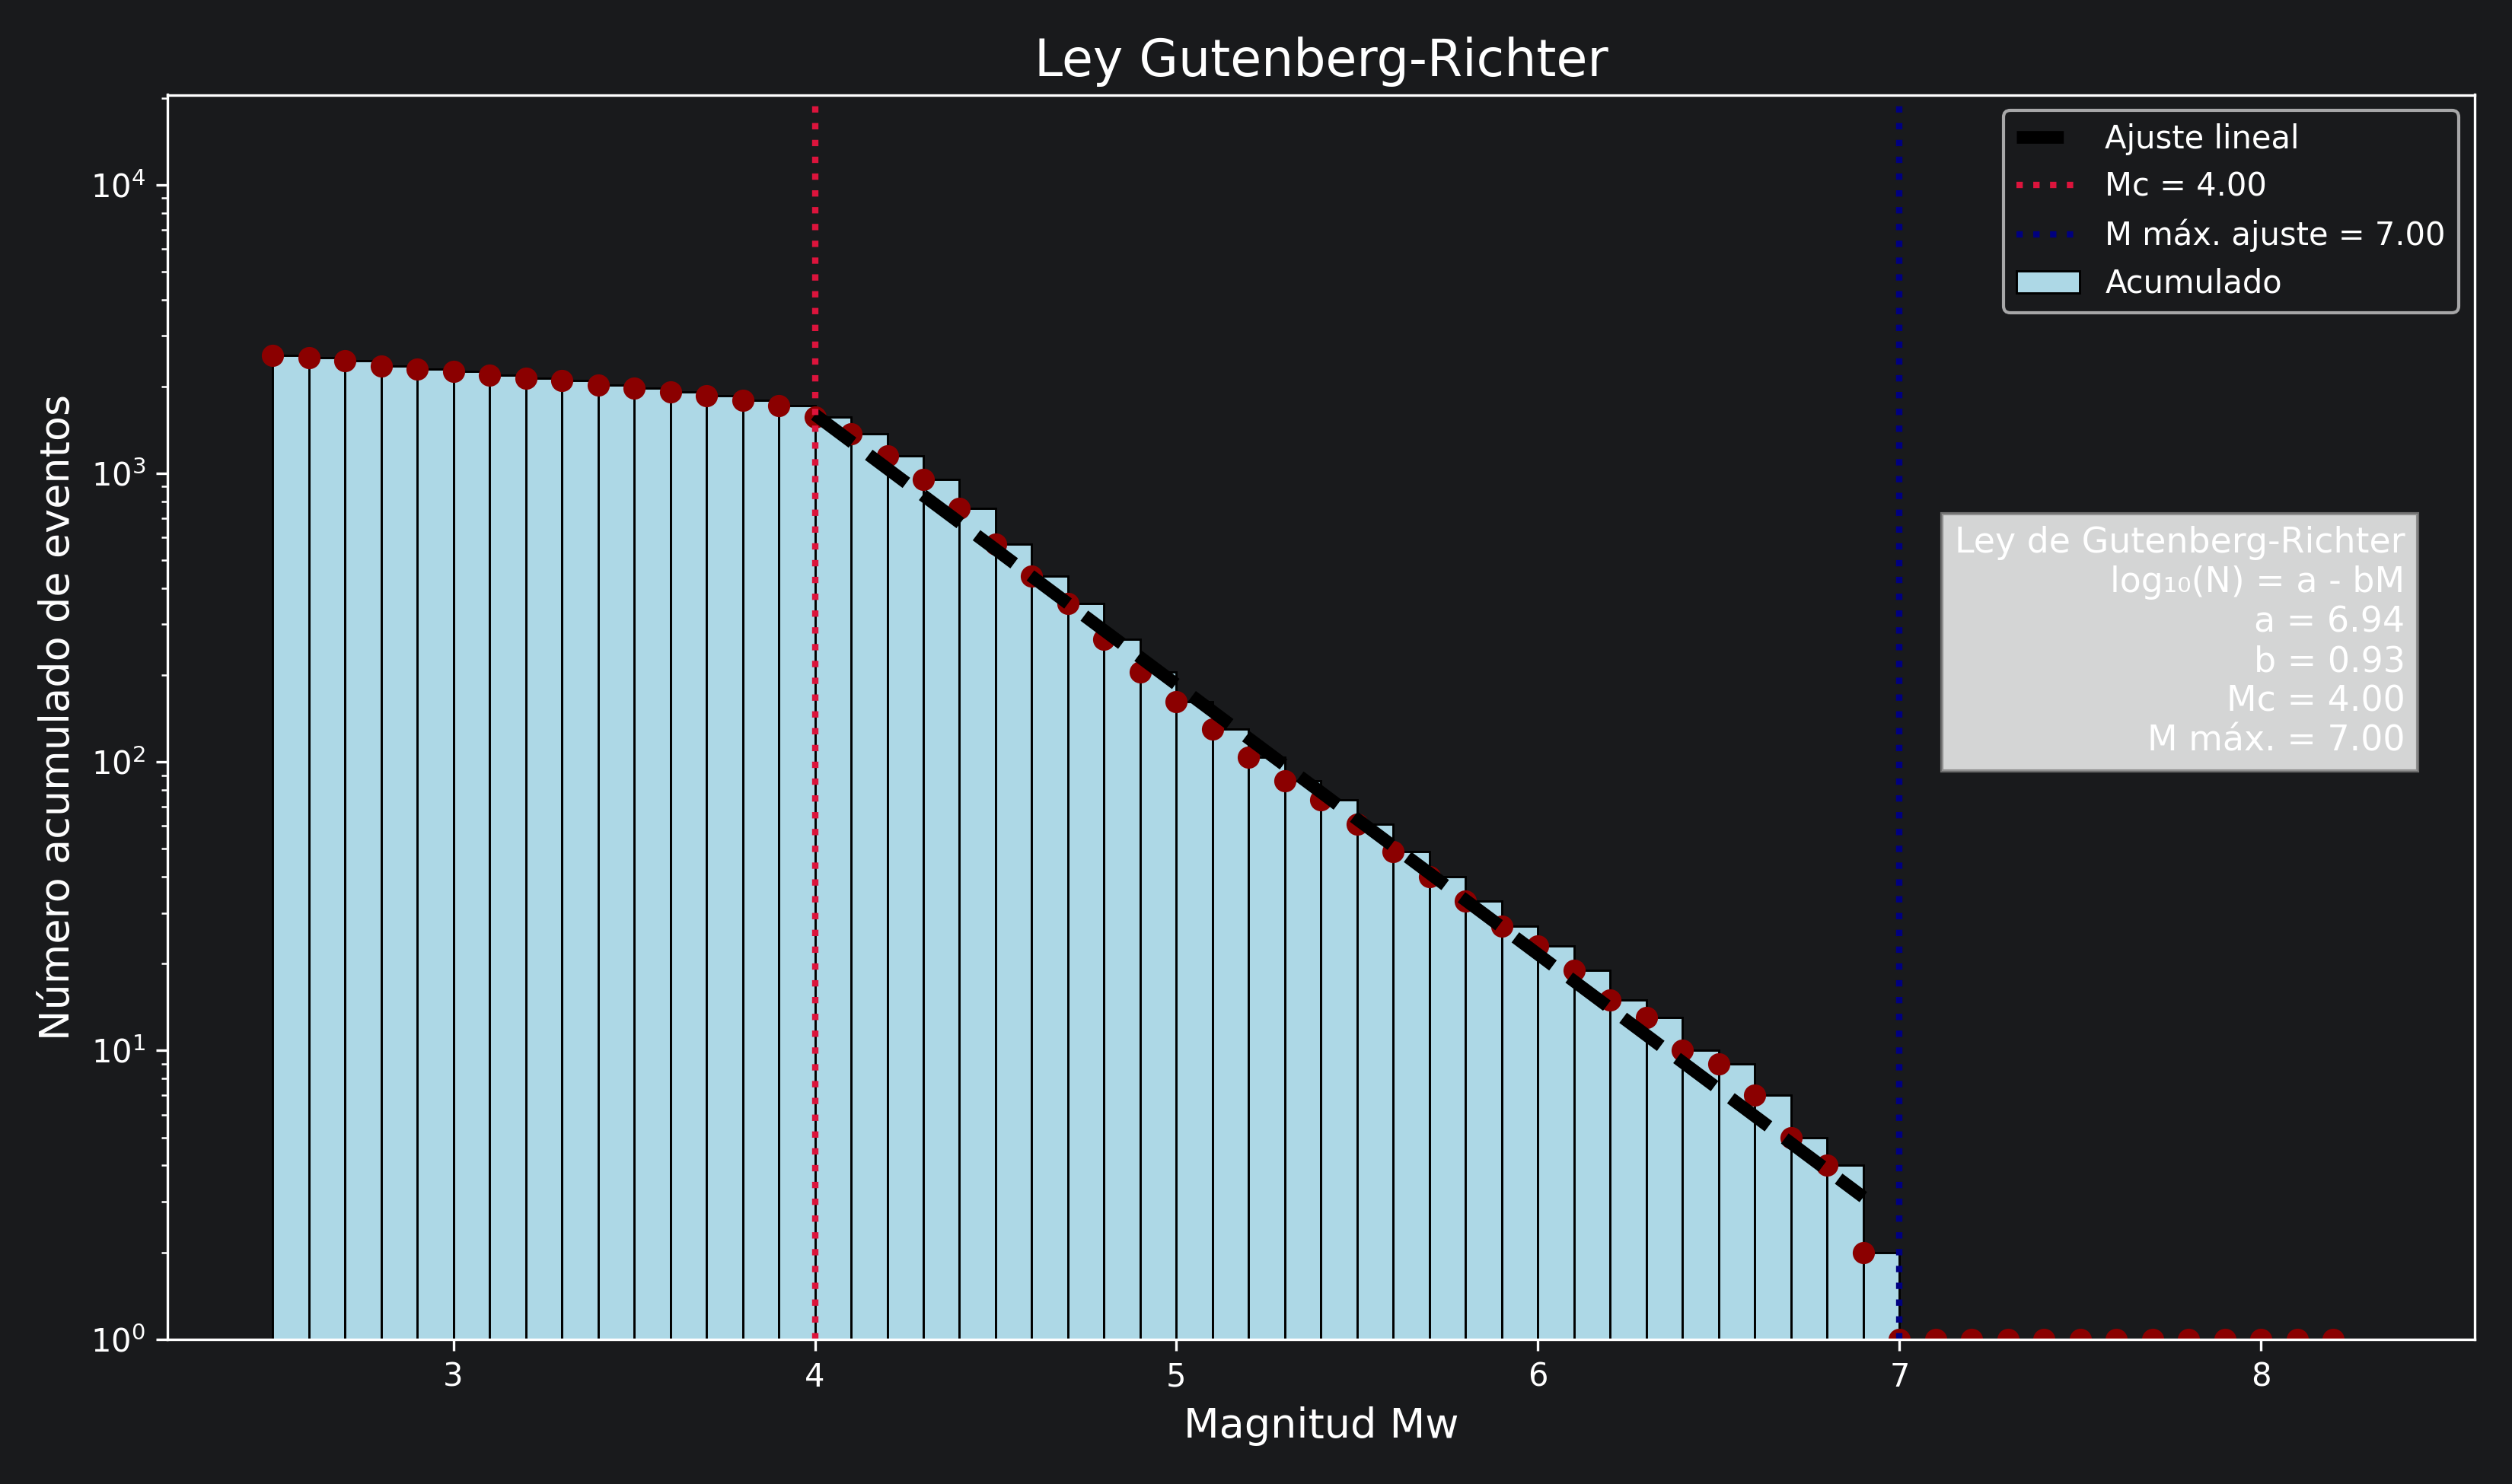
\includegraphics[width=\textwidth]{Figures/Ley_GR}
    \caption{Relación frecuencia--magnitud de Gutenberg--Richter para el catálogo sísmico de la región analizada. Las barras celestes representan el número acumulado de eventos; los puntos rojos corresponden a los valores observados; la línea negra discontinua representa el ajuste lineal. La línea roja punteada indica la magnitud de completitud seleccionada, $M_c = 4{,}0$, y la línea azul punteada marca la magnitud máxima incluida en la regresión, $M_w = 7{,}0$.}
    \label{fig:gutenberg-richter}
\end{figure}

Con el fin de caracterizar la relación entre la magnitud de los sismos y su frecuencia de ocurrencia en la región analizada, se aplicó la ley de Gutenberg--Richter al catálogo acumulado de eventos. La Figura~\ref{fig:gutenberg-richter} presenta el número acumulado de sismos en función de la magnitud Mw en escala logarítmica, junto con el intervalo seleccionado para el ajuste lineal. De acuerdo con la metodología definida previamente, se utilizó una magnitud de completitud de $M_c = 4{,}0$ y se restringió el ajuste al intervalo $4{,}0 \leq M_w \leq 7{,}0$, excluyendo el evento principal de Mw~8{,}3 para evitar que un valor extremo y aislado afectara la estimación de la pendiente.

La figura muestra que, a partir de $M_c = 4{,}0$, la distribución acumulada presenta un comportamiento aproximadamente lineal en el espacio $\log_{10}(N)$--$M_w$, lo que indica que el catálogo es adecuado para aplicar la relación empírica en dicho rango. El ajuste obtenido presenta un parámetro $a = 6{,}94$ y un valor $b = 0{,}93$. El valor de $b$, cercano a la unidad, indica que por cada aumento de una unidad de magnitud, el número acumulado de eventos disminuye aproximadamente en un orden de magnitud.

Por lo tanto, la ecuación de mejor ajuste para la región y período de estudio es:

\[
\log_{10}\left(N\right) = 6{,}94 - 0{,}93M_w,
\]

donde $N$ corresponde al número acumulado de eventos con magnitud igual o superior a $M_w$.

Esta expresión resume la distribución frecuencia--magnitud del catálogo analizado y constituye una base cuantitativa para interpretar la proporción relativa entre sismos moderados y eventos de mayor magnitud.

\subsubsection{¿Qué información nos revela el valor del parámetro a y b en la Ley de Gutenberg-Richter sobre
el Peligro Sísmico de la zona?}
El parámetro $a = 6{,}94$ representa el nivel global de actividad sísmica del catálogo dentro del intervalo temporal, espacial y de magnitudes seleccionado. Un valor elevado de $a$ indica que, para una magnitud de referencia, la región presenta una cantidad importante de eventos acumulados, es decir, refleja una zona seleccionada tectónicamente activa. Sin embargo, este parámetro depende también del tamaño del área analizada, de la duración del catálogo y de la magnitud de completitud utilizada, por lo que debe interpretarse principalmente como un indicador relativo de la productividad sísmica y no como una medida aislada del peligro.

Por otro lado, el parámetro $b = 0{,}93$ corresponde a la pendiente de la relación frecuencia--magnitud y expresa la proporción entre sismos pequeños y grandes. Al ser cercano a uno, indica que por cada incremento de una unidad en la magnitud Mw, el número acumulado de eventos disminuye aproximadamente por un factor de:

\[
10^{0{,}93} \approx 8{,}5.
\]

En consecuencia, los terremotos de gran magnitud son mucho menos frecuentes que los eventos moderados o pequeños, pero no están ausentes en el comportamiento estadístico de la región.

Desde la perspectiva del peligro sísmico, la combinación de un valor alto de $a$ y un valor de $b$ cercano a la unidad indica una región con actividad alta y una disminución regular, pero no excesivamente rápida, de la ocurrencia al aumentar la magnitud. Por lo tanto, la zona tiene una alta recurrencia de sismos de menor y mediana magnitud y mantiene una probabilidad no despreciable de generar terremotos fuertes.

\subsection{Ley de Omori}
La Ley de Omori describe la variación temporal de la actividad sísmica después de un evento principal. Su forma general es:

\[
n(t) = \frac{K}{(t + c)^p}
\]

donde $n(t)$ es el número de aftershocks en el tiempo $t$, $K$, $c$ y $p$ son parámetros que dependen del evento principal y del entorno geológico.

\begin{figure}[]
    \centering
    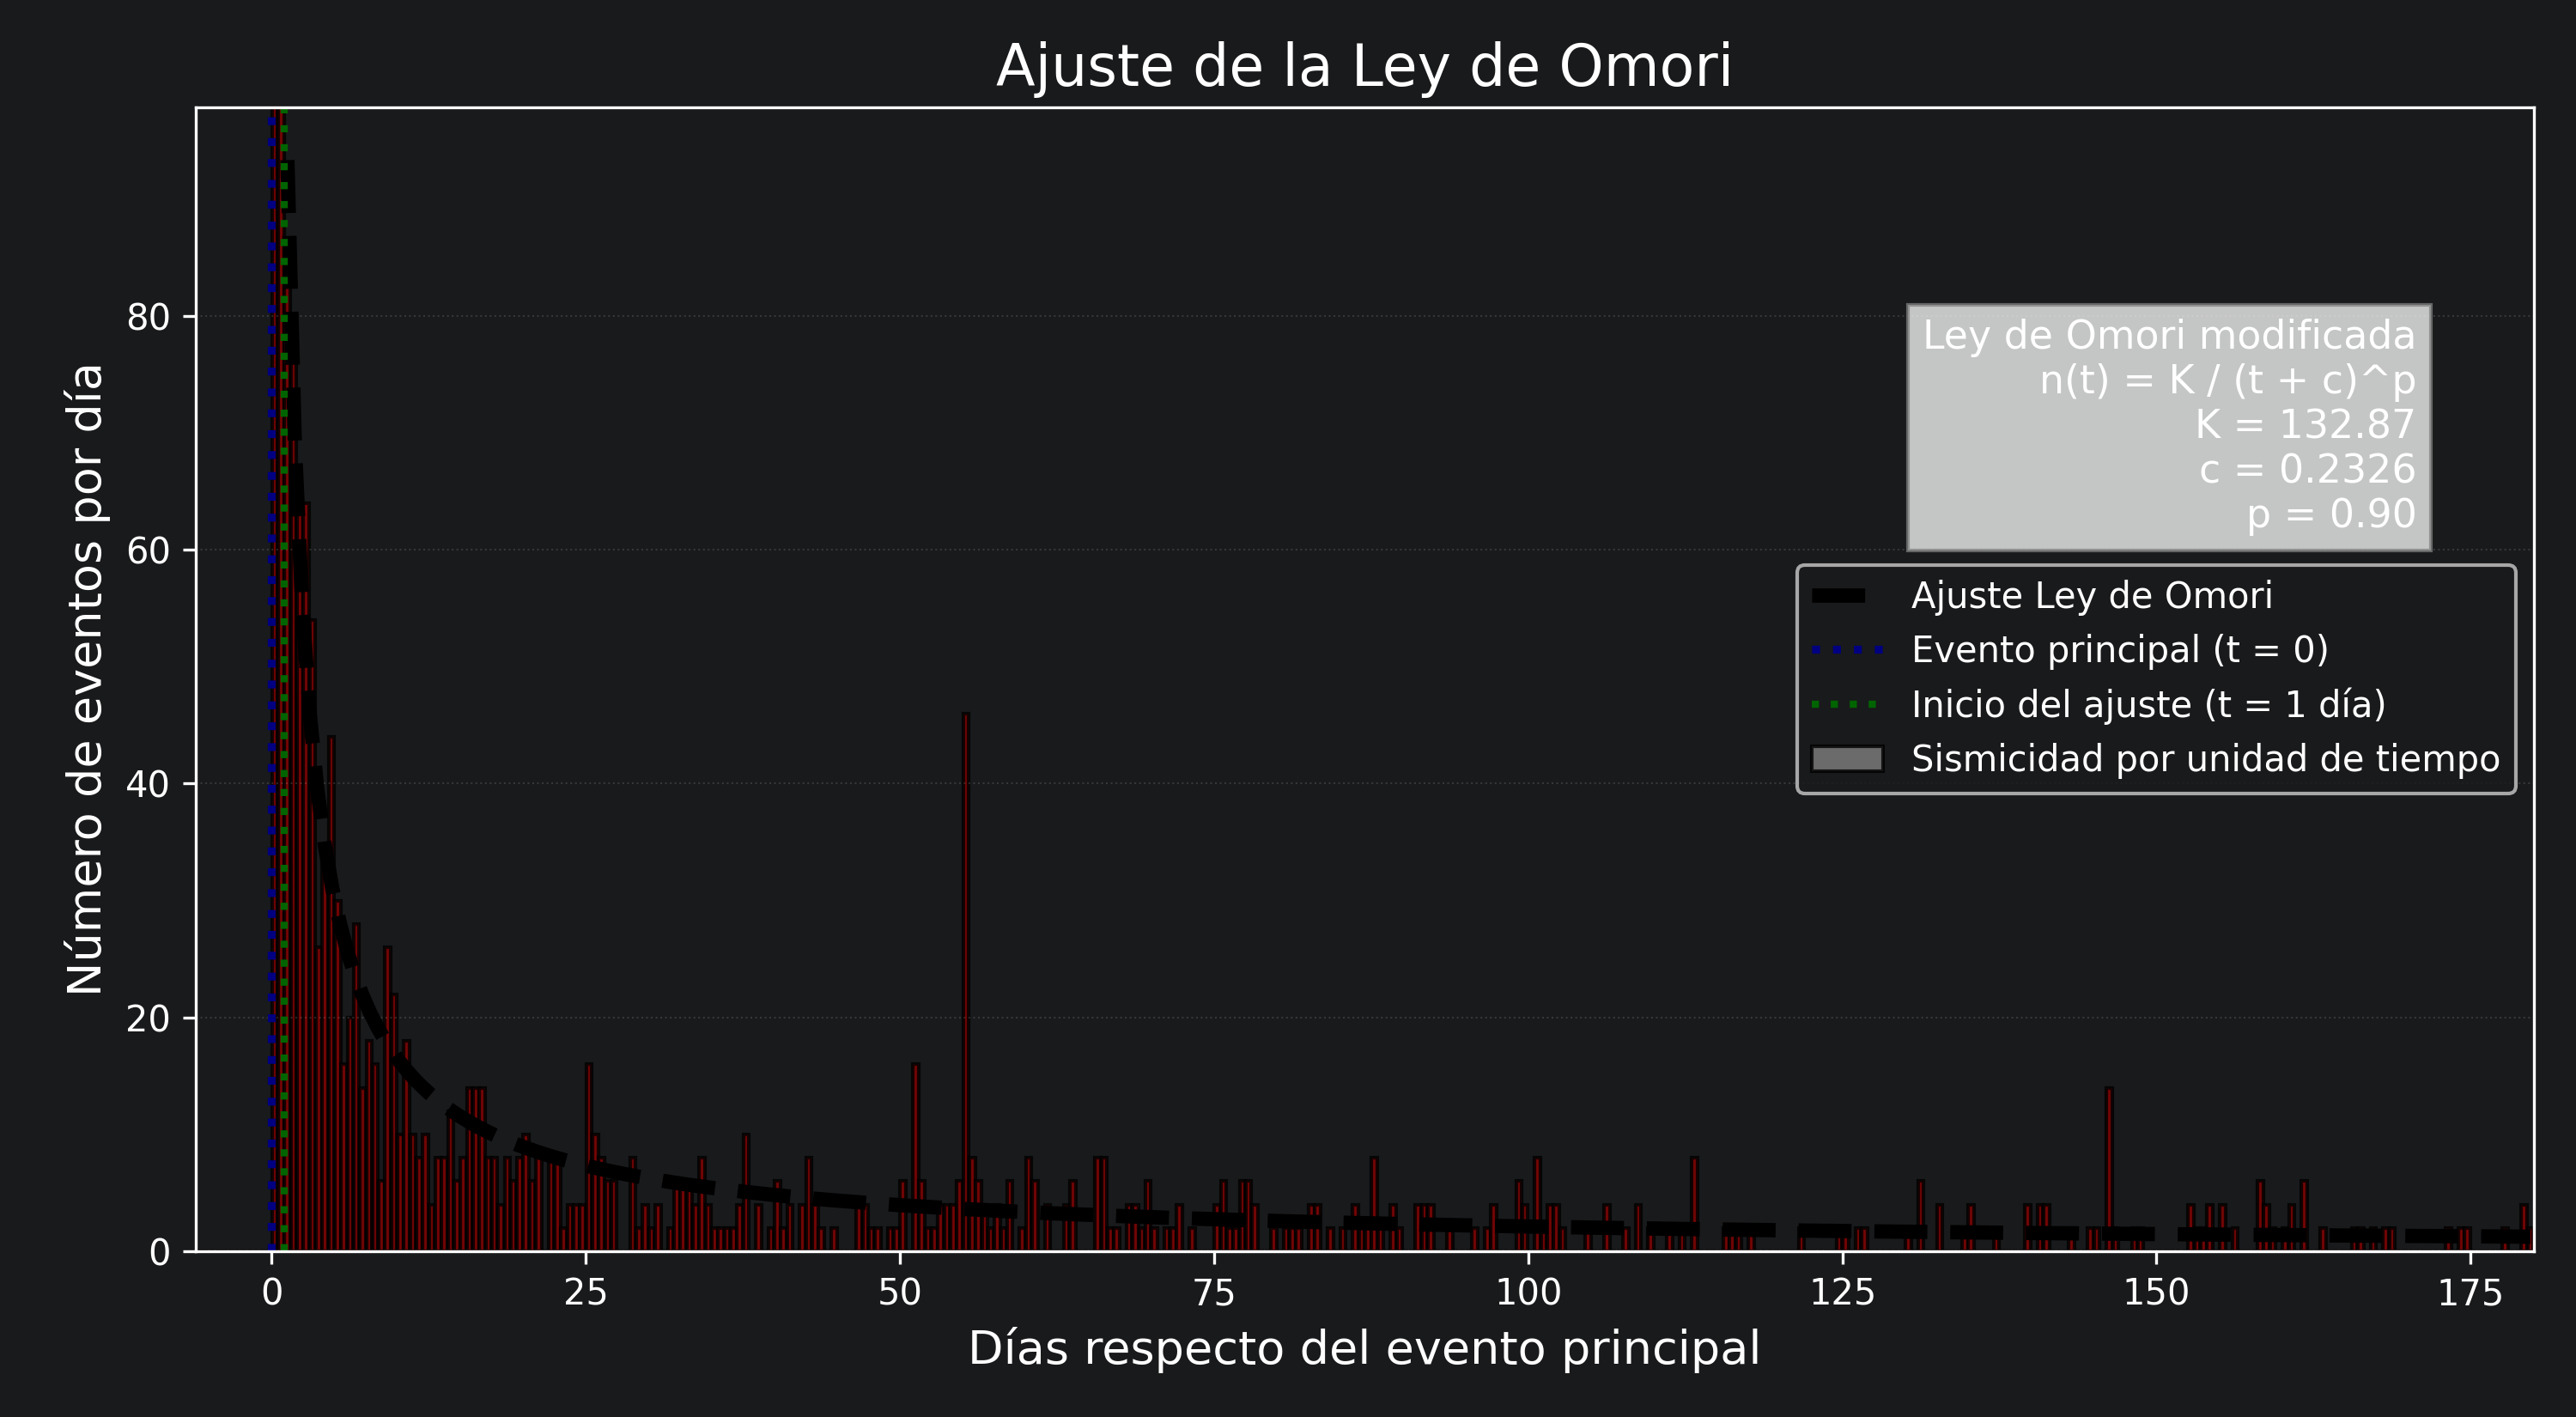
\includegraphics[width=\textwidth]{Figures/Omori}
    \caption{Ajuste de la ley de Omori modificada para la secuencia de réplicas posterior al evento principal de Mw~8{,}3. Las barras representan el número de eventos por unidad de tiempo; la línea negra discontinua corresponde al ajuste no lineal de la ley de Omori. La línea azul punteada indica el instante del evento principal ($t=0$) y la línea verde punteada marca el inicio del intervalo utilizado para el ajuste ($t=1$ día).}
    \label{fig:omori}
\end{figure}

Con el objetivo de caracterizar la evolución temporal de las réplicas asociadas al evento principal de magnitud Mw~8{,}3 incluido en el catálogo, se aplicó la ley de Omori modificada a la secuencia de réplicas posterior al sismo de Illapel. La Figura~\ref{fig:omori} muestra el número de eventos por unidad de tiempo en función de los días transcurridos desde el terremoto principal, definido como $t=0$. Tal como se mencionó en la sección de metodología, el ajuste se inició a partir de $t=1$ día y se utilizaron bins temporales de 0{,}5 días, con el fin de representar adecuadamente la alta tasa de réplicas inmediatamente después del evento y su posterior disminución.

La figura \ref{fig:omori} evidencia una concentración muy alta de eventos durante los primeros días posteriores al terremoto, con tasas cercanas a 100 eventos por día. Posteriormente, la tasa de sismicidad disminuye de forma rápida durante las primeras semanas y continúa decreciendo de manera más gradual hacia tiempos mayores. Aunque se observan aumentos puntuales de actividad, particularmente alrededor de los días 25, 50 y 145, la tendencia general sigue un decaimiento temporal compatible con la ley de Omori modificada.

El ajuste no lineal de la secuencia de réplicas permitió estimar los parámetros $K = 132{,}87$, $c = 0{,}2326$ y $p = 0{,}90$. Por tanto, la ecuación de mejor ajuste obtenida para la tasa temporal de réplicas es:

\[
n(t) =
\frac{132{,}87}
{\left(t + 0{,}2326\right)^{0{,}90}},
\]

donde $n(t)$ corresponde al número de eventos por día y $t$ representa el tiempo, en días, transcurrido desde el evento principal.

El valor de $p$ cercano a uno indica que la tasa de réplicas disminuye aproximadamente de forma inversamente proporcional al tiempo, mientras que el parámetro $c$ permite representar el comportamiento durante los primeros instantes de la secuencia, evitando una singularidad matemática en $t=0$.

La selección del intervalo temporal para el ajuste de la ley de Omori fue relativamente sencilla en cuanto a la identificación del evento principal, debido a que el terremoto de Mw~8{,}3 destaca claramente como el evento de mayor magnitud del catálogo. Sin embargo, la definición del período útil de análisis requirió considerar que durante las primeras horas posteriores al sismo la tasa de eventos es muy alta y pueden existir fallas en la detección de réplicas. Por esta razón, el ajuste se inició a partir de $t=1$ día.

De igual forma, se hizo uso de información externa acerca de la duración aproximada de las réplicas, por lo que se concluyó que una ventana de aproximadamente 180 días es lo suficientemente extensa para observar el decaimiento de la tasa de réplicas, pero con el costo de secuencias posteriores no relacionadas directamente con el evento principal, como las que se observan alrededor de los días 25, 50 y 145 \cite{Aranguiz_Geotech_Illapel2015}.

\subsection{¿Es posible relacionar las constantes de ambas leyes (Gutenberg-Richter y Omori) para caracterizar una zona sísmica específica?}

Sí, es posible relacionar las constantes de ambas leyes para obtener una caracterización más completa de una zona sísmica, aunque no existe una equivalencia directa y universal entre ellas. Como mencioné antes, la ley de Gutenberg--Richter describe cómo se distribuyen los eventos según su magnitud mediante los parámetros $a$ y $b$, mientras que la ley de Omori caracteriza la evolución temporal de una secuencia de réplicas mediante $K$, $c$ y $p$.

Así como se mencionó antes, el valor $a=6{,}94$ indica una actividad sísmica acumulada importante en el catálogo de la region de subducción de Chile y $b=0{,}93$ describe una disminución cercana a un orden de magnitud en la frecuencia de eventos por cada unidad de aumento en Mw. Por otra parte, los parámetros de Omori, $K=132{,}87$, $c=0{,}2326$ y $p=0{,}90$, caracterizan una secuencia de réplicas inicialmente muy productiva y con una disminución temporal cercana a una relación inversa con el tiempo. La relación entre estos conjuntos de parámetros permite describir simultáneamente dos dimensiones de la actividad sísmica: La frecuencia relativa de eventos pequeños y grandes, dada por $a$ y $b$, y la duración e intensidad temporal de la actividad posterior a un terremoto principal, dada por $K$, $c$ y $p$.

Un gran ejemplo de relacionamiento de dicha información reside en modelos de pronóstico de réplicas, como el modelo de Reasenberg--Jones o los modelos ETAS. En donde integrando los parámetros estimados de ambas leyes es posible estimar la tasa esperada de eventos de una magnitud mínima durante un intervalo temporal posterior a un sismo principal. Por lo que se puede concluir que, de nuevo, si es posible caracterizar mejor una zona sísmica uniendo la información de dichas fuentes.

\newpage
\section{Conclusiones}

El análisis del catálogo sísmico del segmento Coquimbo--Illapel, comprendido aproximadamente entre $29^\circ$S y $33^\circ$S, $69^\circ$W y $73^\circ$W, para el período 2007--2017, permitió caracterizar la actividad sísmica asociada al margen de subducción entre las placas de Nazca y Sudamericana. El catálogo, compuesto por 2563 eventos con magnitudes entre Mw~2{,}5 y Mw~8{,}3, evidenció una concentración principal de sismicidad próxima a la costa y a la zona de contacto entre ambas placas. La selección de una sección transversal A--B, aproximadamente este--oeste y perpendicular al margen, permitió representar de manera adecuada la variación de la profundidad de los eventos desde el dominio oceánico hacia el continental.

Asímismo, el perfil de profundidad permitió distinguir diferentes regiones sismotectónicos. Se identificó una banda inclinada de eventos compatible con la sismicidad interplaca, asociada a la región de subducción; eventos superficiales costa afuera relacionados con la torsión de la placa oceánica antes de ingresar a la fosa, interpretados como sismicidad \emph{outer--rise}, eventos corticales continentales próximos a la superficie y eventos de mayor profundidad asociados a deformaciones interna de la placa de Nazca subducida. Esta distribución confirma que la sismicidad regional no responde a una única fuente, sino a la interacción de procesos tectónicos que operan en distintos sectores y profundidades del margen.

La cercanía entre la zona de subducción activa y la línea de costa implica una condición relevante de peligro sísmico para las localidades costeras de la región de Coquimbo. Los eventos interplaca de gran magnitud pueden producir movimientos intensos del terreno en áreas pobladas cercanas al litoral y, si generan desplazamientos verticales del fondo marino, pueden originar tsunamis. Por lo tanto, el peligro local depende no sólo de la frecuencia de sismos, sino también de la geometría de la zona de ruptura, la profundidad de los eventos, la distancia a los centros poblados, las condiciones locales de sitio y la exposición al borde costero.

El análisis de latitud versus tiempo mostró una actividad de fondo relativamente dispersa durante gran parte del período de estudio, junto con una concentración excepcional de eventos desde septiembre de 2015. Este aumento corresponde a la secuencia asociada al terremoto de Illapel de Mw~8{,}3 y sus réplicas, visibles como una concentración temporal y espacial entre aproximadamente $29{,}5^\circ$S y $32{,}5^\circ$S. Aunque la figura \ref{fig:perfil-temporal} sugiere una expansión de la actividad hacia segmentos adyacentes al área de ruptura, no permite establecer una migración latitudinal única y sostenida. Asimismo, los intervalos de menor actividad registrados antes de 2015 deben interpretarse con cautela, pues la menor cantidad de eventos observados no implica necesariamente una disminución del peligro sísmico, aunque sí representa un ejemplo del cíclo sísmico de dichas regiones de subducción.

La relación frecuencia--magnitud del catálogo se ajustó satisfactoriamente mediante la ley de Gutenberg--Richter en el intervalo $4{,}0 \leq M_w \leq 7{,}0$, utilizando una magnitud de completitud de $M_c=4{,}0$. El ajuste obtenido fué:

\[
\log_{10}\left(N\right) = 6{,}94 - 0{,}93M_w.
\]

Donde el parámetro $a=6{,}94$ refleja una productividad sísmica importante para el catálogo y región analizados, mientras que el valor $b=0{,}93$, cercano a uno, indica una disminución regular de la frecuencia de sismos al aumentar la magnitud. En términos de peligro sísmico, estos resultados evidencian una alta recurrencia de eventos pequeños y moderados, sin descartar la posibilidad de terremotos fuertes, como el evento de Illapel incluido en el catálogo.

Por otra parte, la secuencia de réplicas posterior al terremoto principal se ajustó mediante la ley de Omori modificada, usando bins temporales de 0{,}5 días, un inicio de ajuste desde $t=1$ día y una ventana de análisis de aproximadamente 180 días. La ecuación obtenida fué, respectivamente:

\[
n(t) =
\frac{132{,}87}
{\left(t+0{,}2326\right)^{0{,}90}}.
\]

En donde los parámetros estimados, $K=132{,}87$, $c=0{,}2326$ y $p=0{,}90$, describen una tasa inicial elevada de réplicas y un decaimiento temporal cercano a una relación inversa con el tiempo. Si bien se identificaron aumentos puntuales de sismicidad durante la ventana analizada, la tendencia general fue consistente con el comportamiento esperado para una secuencia de réplicas posterior a un gran terremoto interplaca.

Finalmente, los resultados de Gutenberg--Richter y Omori son complementarios para la caracterización de la zona sísmica de la costa de Coquimbo. Los parámetros $a$ y $b$ describen la distribución de los eventos según su magnitud en el catálogo regional, mientras que $K$, $c$ y $p$ representan la productividad y evolución temporal de una secuencia de réplicas particular. Aunque no existe una relación directa y universal entre ambos grupos de constantes, su integración permite describir tanto la frecuencia relativa de eventos de diferente magnitud como la evolución temporal esperable después de un terremoto principal. En consecuencia, el análisis conjunto de la geometría de la subducción, la distribución espacial y temporal de los eventos, y las leyes empíricas aplicadas constituye una base útil para la evaluación inicial del peligro sísmico en el margen chileno central.
\newpage

\clearpage
\newpage
\bibliographystyle{IEEEtran}
\bibliography{sample}
\end{document}